\section{System Design and Architecture}

\subsection{High-Level Architecture}
The system is designed as a two-layer architecture that separates content generation from content delivery.

\begin{itemize}
    \item \textbf{Layer A — generation pipeline:} custom parsers load configuration and media inputs, while the engine orchestrates synchronization and frame-by-frame ASCII rendering.
    \item \textbf{Layer B — delivery pipeline:} rendered frames are compressed into a compact file format, then replayed through a preview path that reconstructs and displays frames.
\end{itemize}

This separation improves maintainability and directly supports user-facing needs: high-fidelity raw output for inspection and compressed output for practical storage and playback.

\subsection{Module Hierarchy}
The repository is organized around clear functional boundaries:

\begin{itemize}
    \item \textbf{Parser modules} (\url{src/parsers}): JSON/config parsing, WAV parsing, and BMP parsing.
    \item \textbf{Engine and rendering modules} (\url{src/components}): sequence path logic, ASCII conversion, rendering, compressed render I/O, and engine orchestration.
    \item \textbf{Compression modules} (\url{src/compressions}): compression/decompression dispatch and algorithm implementations (\url{none}, \texttt{rle}, \texttt{delta}, \texttt{huffman}).
    \item \textbf{Public interfaces} (\url{include/...}): typed APIs and shared data structures per subsystem.
    \item \textbf{Validation modules} (\url{tests/...}): subsystem-level tests for parser, component, and compression behavior.
\end{itemize}

The resulting hierarchy keeps file-format concerns, orchestration logic, and storage optimization logic decoupled while still integrating through explicit interfaces.

\subsection{End-to-End Data Flow}
At runtime, the engine consumes three inputs:
\begin{enumerate}[label=\arabic*)]
    \item JSON configuration (frame range, frame naming rules, palette, threshold, compression settings);
    \item WAV audio stream;
    \item BMP frame sequence.
\end{enumerate}

The engine first validates and prepares context (configuration, audio metadata, frame range), then processes each frame by loading image data, mapping it to the corresponding audio interval, rendering ASCII, and writing outputs. The system produces:
\begin{itemize}
    \item raw ASCII render text;
    \item compressed frame output;
    \item process log for traceability and debugging.
\end{itemize}

The preview program then reads the compressed output file, reconstructs compression context (including Huffman FSM metadata when applicable), decompresses frame payloads, and prints animated ASCII to the terminal.

\begin{figure}[H]
    \centering
    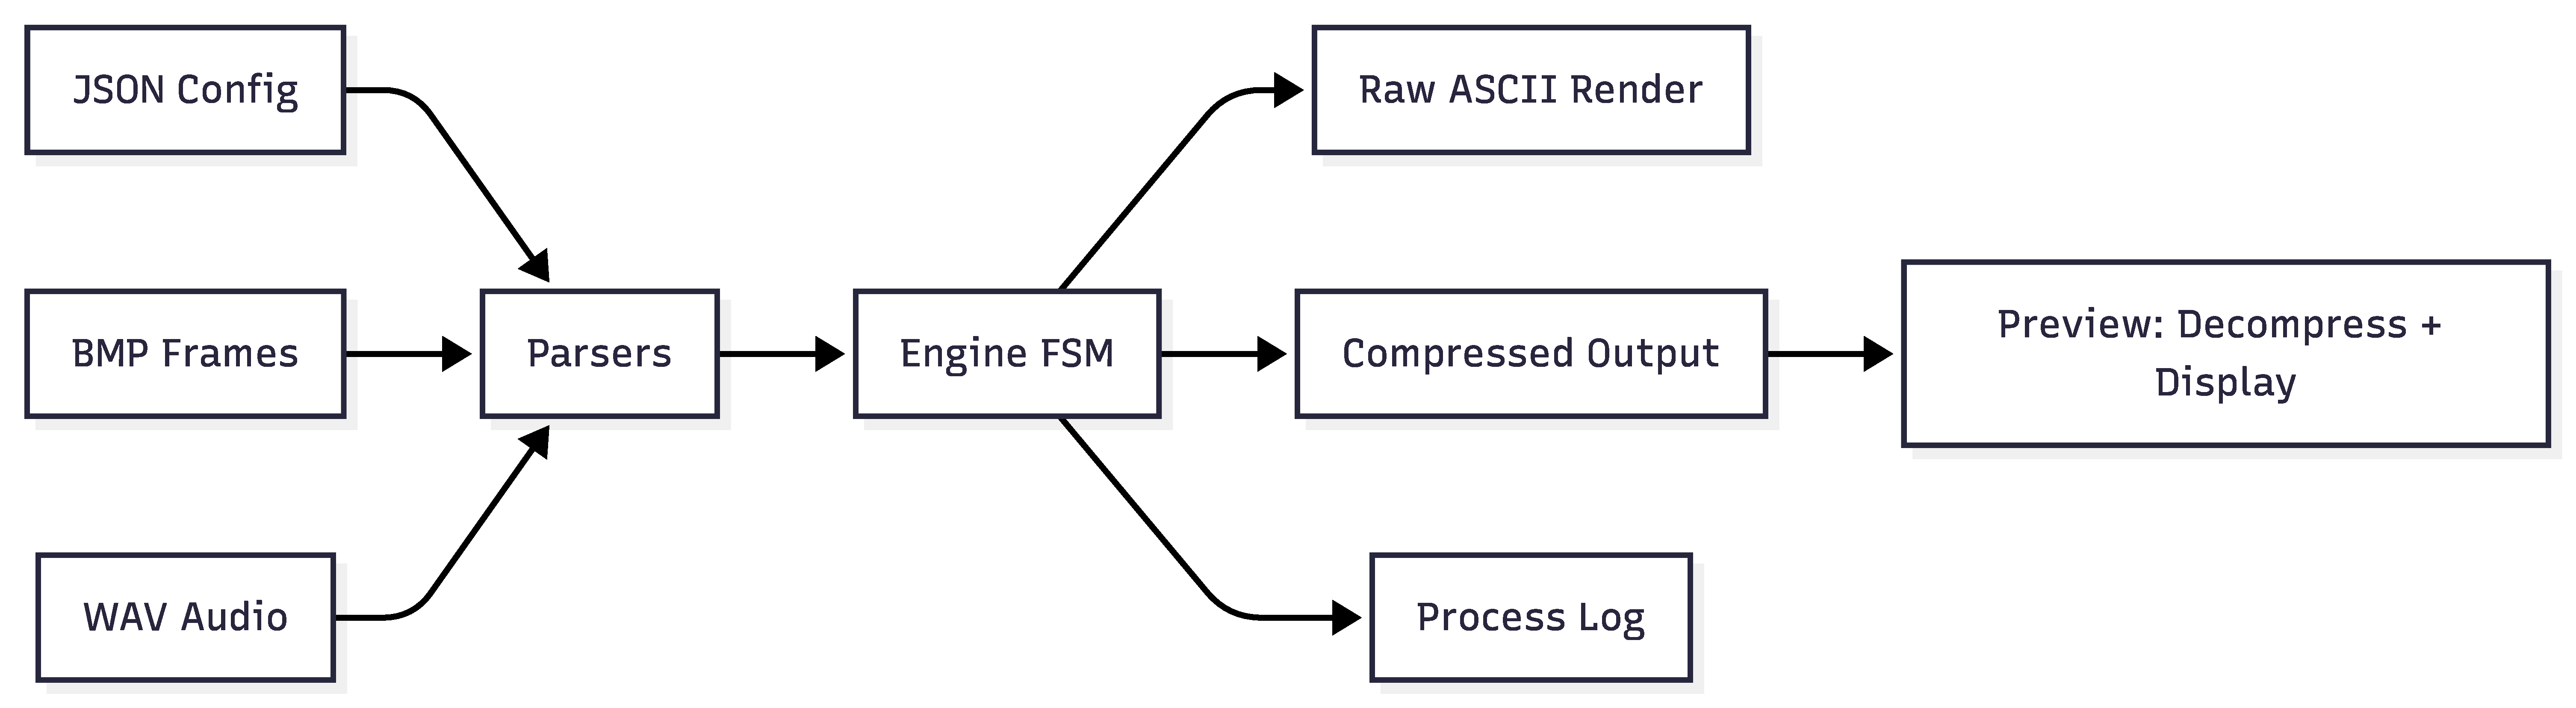
\includegraphics[width=0.75\textwidth]{figures/detailed_architecture.pdf}
    % flowchart LR
    % A[JSON Config] --> D[Parsers]
    % B[BMP Frames] --> D
    % C[WAV Audio] --> D
    % D --> E[Engine FSM]
    % E --> F[Raw ASCII Render]
    % E --> G[Compressed Output]
    % E --> H[Process Log]
    % G --> I[Preview: Decompress + Display]
    \caption{End-to-end architecture from heterogeneous inputs to user-facing outputs.}
    \label{fig:architecture_flow_placeholder}
\end{figure}

\subsection{State-Machine Orchestration}
The core orchestrator is implemented as a deterministic finite state machine in the engine. The major states are:
\texttt{LOAD\_CONFIG}, \texttt{LOAD\_WAV}, \texttt{PREPARE\_SEQUENCE}, \texttt{COLLECT\_STAT}, \texttt{PREPARE\_COMPRESSION}, \texttt{OPEN\_OUTPUTS}, \texttt{PROCESS\_FRAME}, and \texttt{WRITE\_SUMMARY}, with terminal states \texttt{DONE} and \texttt{ERROR}.

Two design choices are important:
\begin{itemize}
    \item \textbf{Pre-processing for compression readiness:} the \texttt{COLLECT\_STAT} and \texttt{PREPARE\_COMPRESSION} stages prepare codec-specific context (notably Huffman symbol statistics and FSM tables) before frame emission.
    \item \textbf{Fail-fast transitions:} any stage-level failure transitions directly to \texttt{ERROR}, providing clear control flow and predictable cleanup behavior.
\end{itemize}

This FSM-centric structure improves readability, isolates stage responsibilities, and supports robust error propagation across heterogeneous processing steps.

\begin{figure}[H]
    \centering
    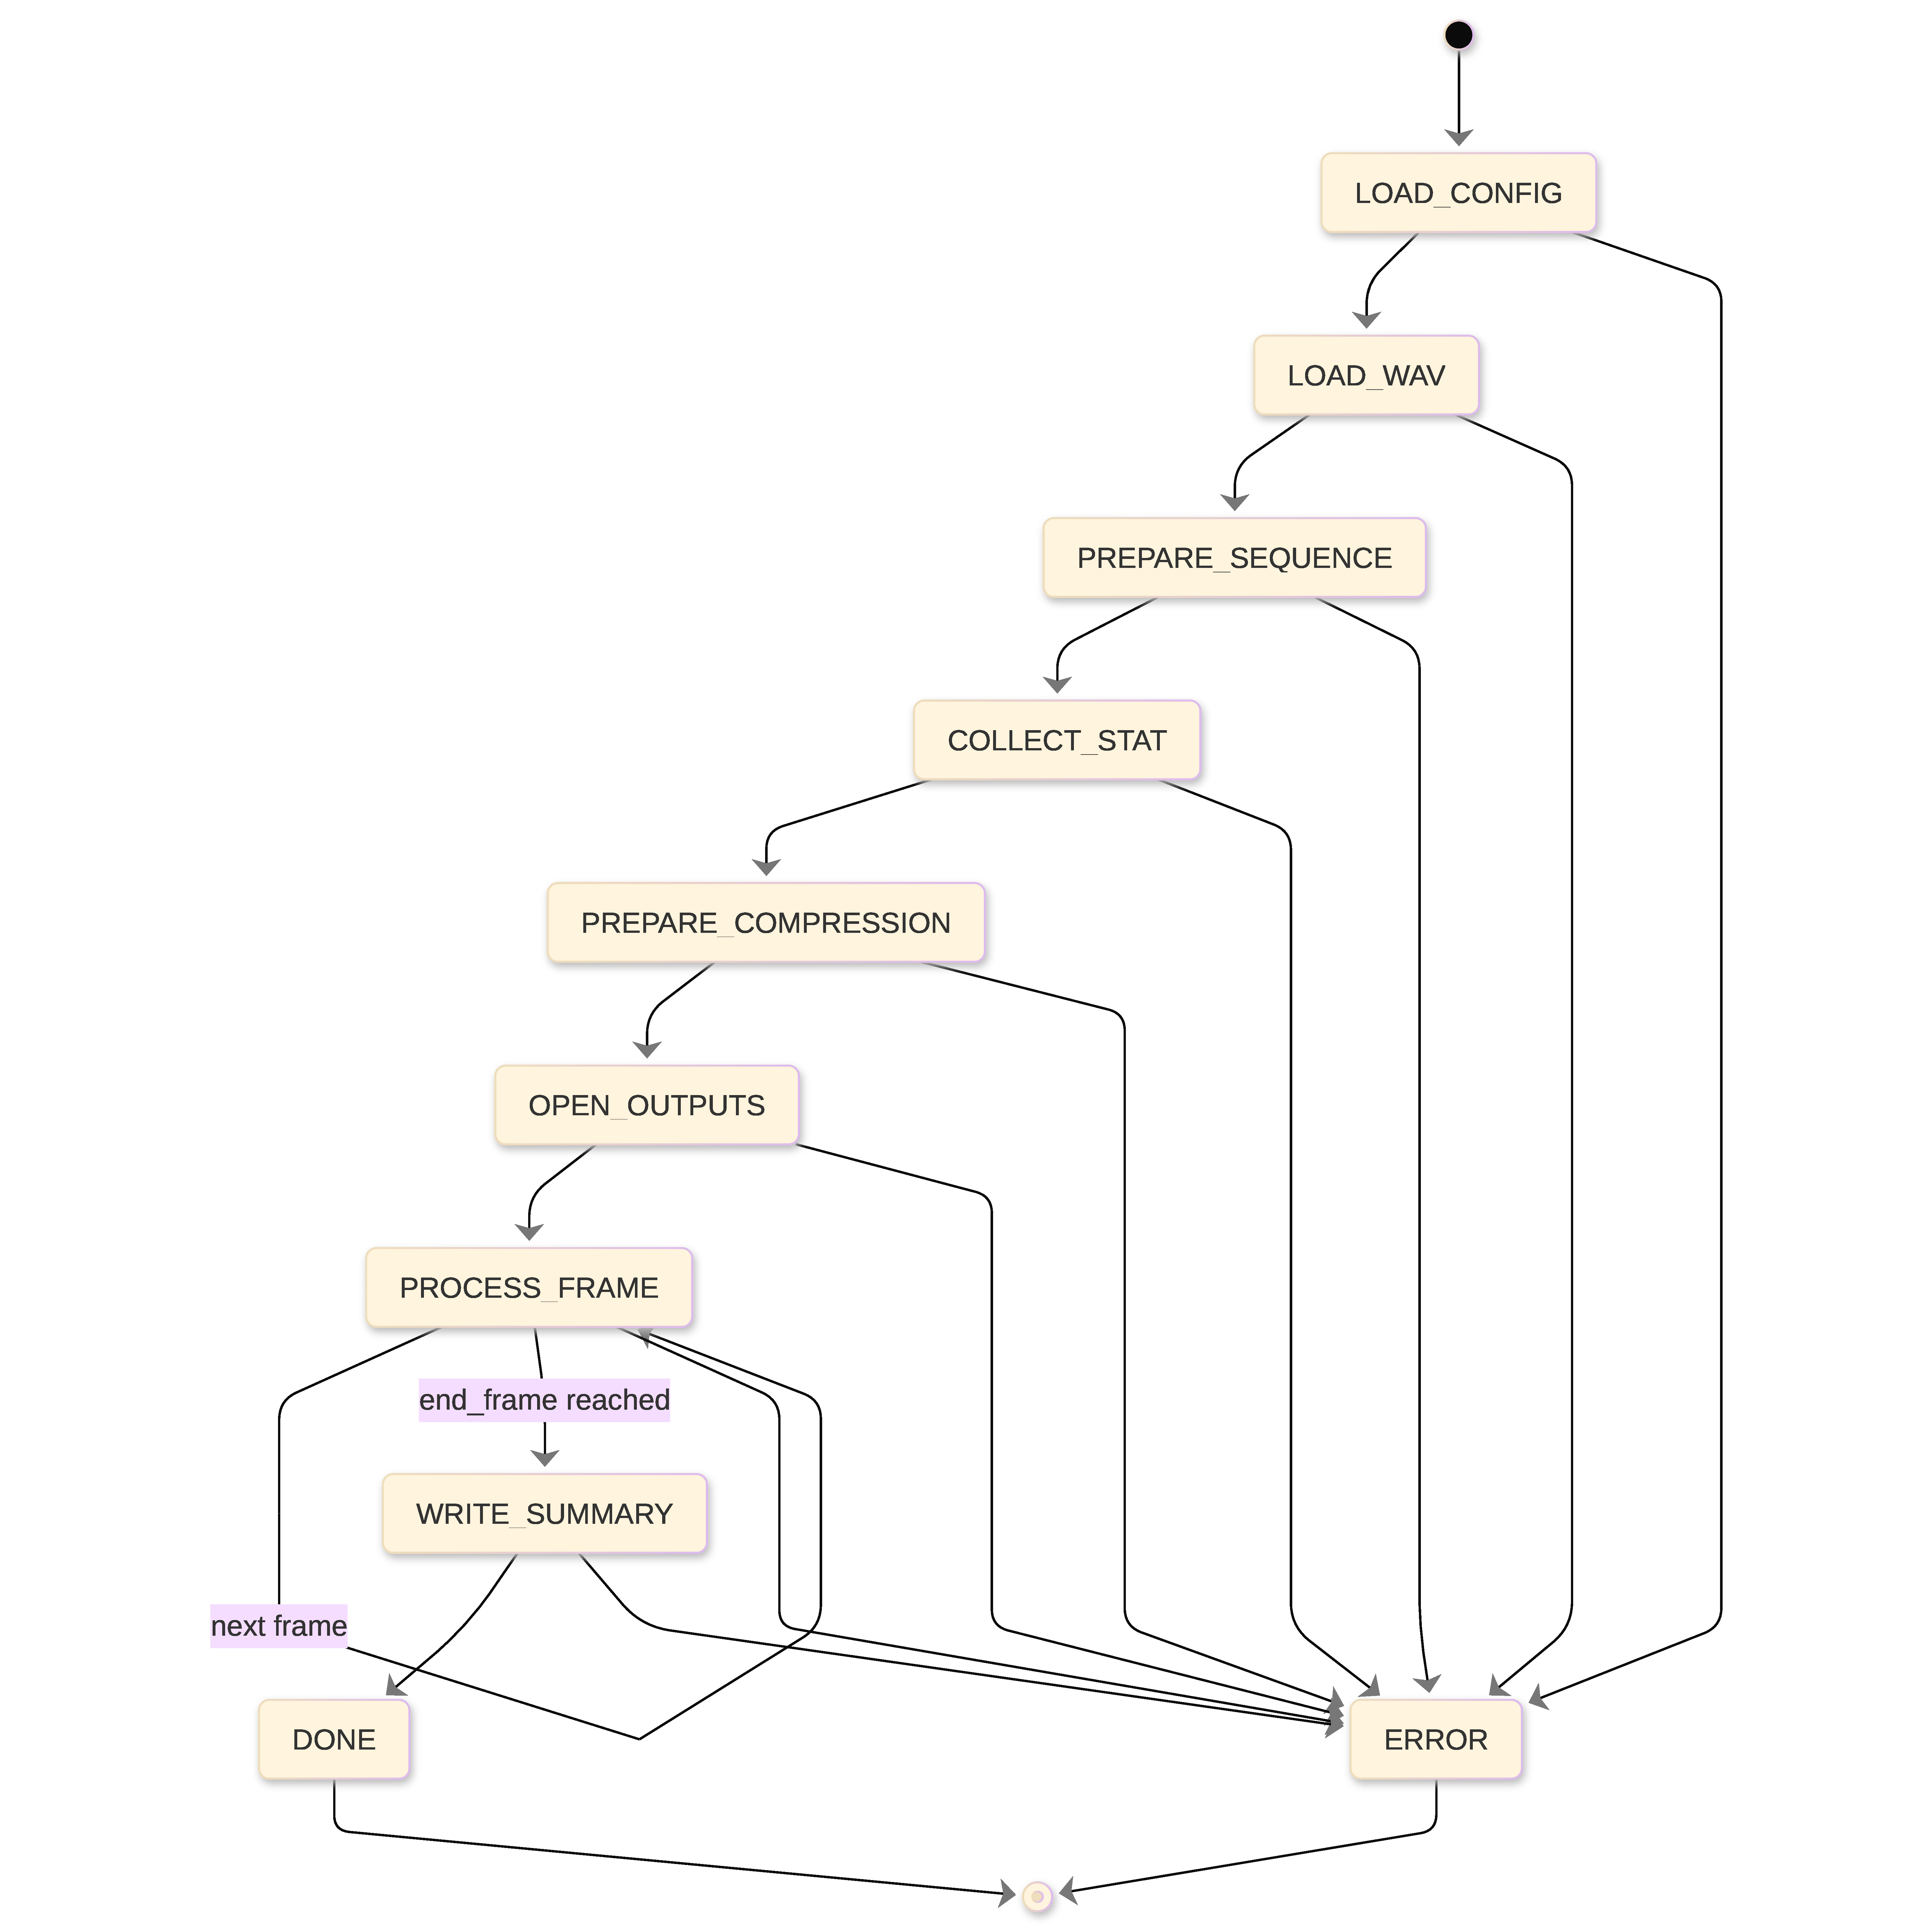
\includegraphics[width=0.75\textwidth]{figures/main_engine_fsm.pdf}
    % ---
    % config:
    % theme: base
    % ---
    % stateDiagram-v2
    % [*] --> LOAD_CONFIG
    % LOAD_CONFIG --> LOAD_WAV
    % LOAD_WAV --> PREPARE_SEQUENCE
    % PREPARE_SEQUENCE --> COLLECT_STAT
    % COLLECT_STAT --> PREPARE_COMPRESSION
    % PREPARE_COMPRESSION --> OPEN_OUTPUTS
    % OPEN_OUTPUTS --> PROCESS_FRAME
    % PROCESS_FRAME --> PROCESS_FRAME: next frame
    % PROCESS_FRAME --> WRITE_SUMMARY: end_frame reached
    % WRITE_SUMMARY --> DONE
    % LOAD_CONFIG --> ERROR
    % LOAD_WAV --> ERROR
    % PREPARE_SEQUENCE --> ERROR
    % COLLECT_STAT --> ERROR
    % PREPARE_COMPRESSION --> ERROR
    % OPEN_OUTPUTS --> ERROR
    % PROCESS_FRAME --> ERROR
    % WRITE_SUMMARY --> ERROR
    % DONE --> [*]
    % ERROR --> [*]
    \caption{State-machine orchestration used by the engine runtime.}
    \label{fig:engine_fsm_placeholder}
\end{figure}

\subsection{Temporal Alignment Logic}
Temporal alignment is handled by mapping each frame's relative index to an audio sample range using configured frames-per-second and WAV sample rate. For frame index $i$, the engine computes:
\begin{equation}
\texttt{start\_sample} = \frac{i \cdot \texttt{sample\_rate}}{\texttt{fps}}, \qquad
\texttt{end\_sample} = \frac{(i+1) \cdot \texttt{sample\_rate}}{\texttt{fps}}.
\end{equation}

The average audio amplitude over this interval drives a highlight decision against a configured threshold. This mechanism ensures that visual emphasis in the ASCII output is synchronized with local audio intensity, producing coherent audio-reactive animation rather than independent frame and sound streams.


\subsection{Compression Algorithms}
To reduce the storage size of the ASCII text files generated by the renderer, several compression algorithms are investigated and implemented. These algorithms are selected to represent different compression paradigms, ranging from simple run-based encoding to probabilistic coding methods.

\subsubsection{Run-Length Encoding (RLE)}
Run-Length Encoding (RLE) is a simple lossless compression technique that reduces redundancy by encoding consecutive repeated characters as a single value and a count. Instead of storing each character individually, RLE represents a sequence as a pair consisting of the character and the number of its repetitions.

\vspace{0.5em}
\noindent\textbf{Example}
$$
AAAAABBBCC \xrightarrow{\text{RLE encode}} A5B3C2 
$$

\vspace{0.5em}
\noindent\textbf{FSMs}
\begin{figure}[H]
    \centering
    
    \begin{subfigure}[t]{0.48\linewidth}
        \centering
        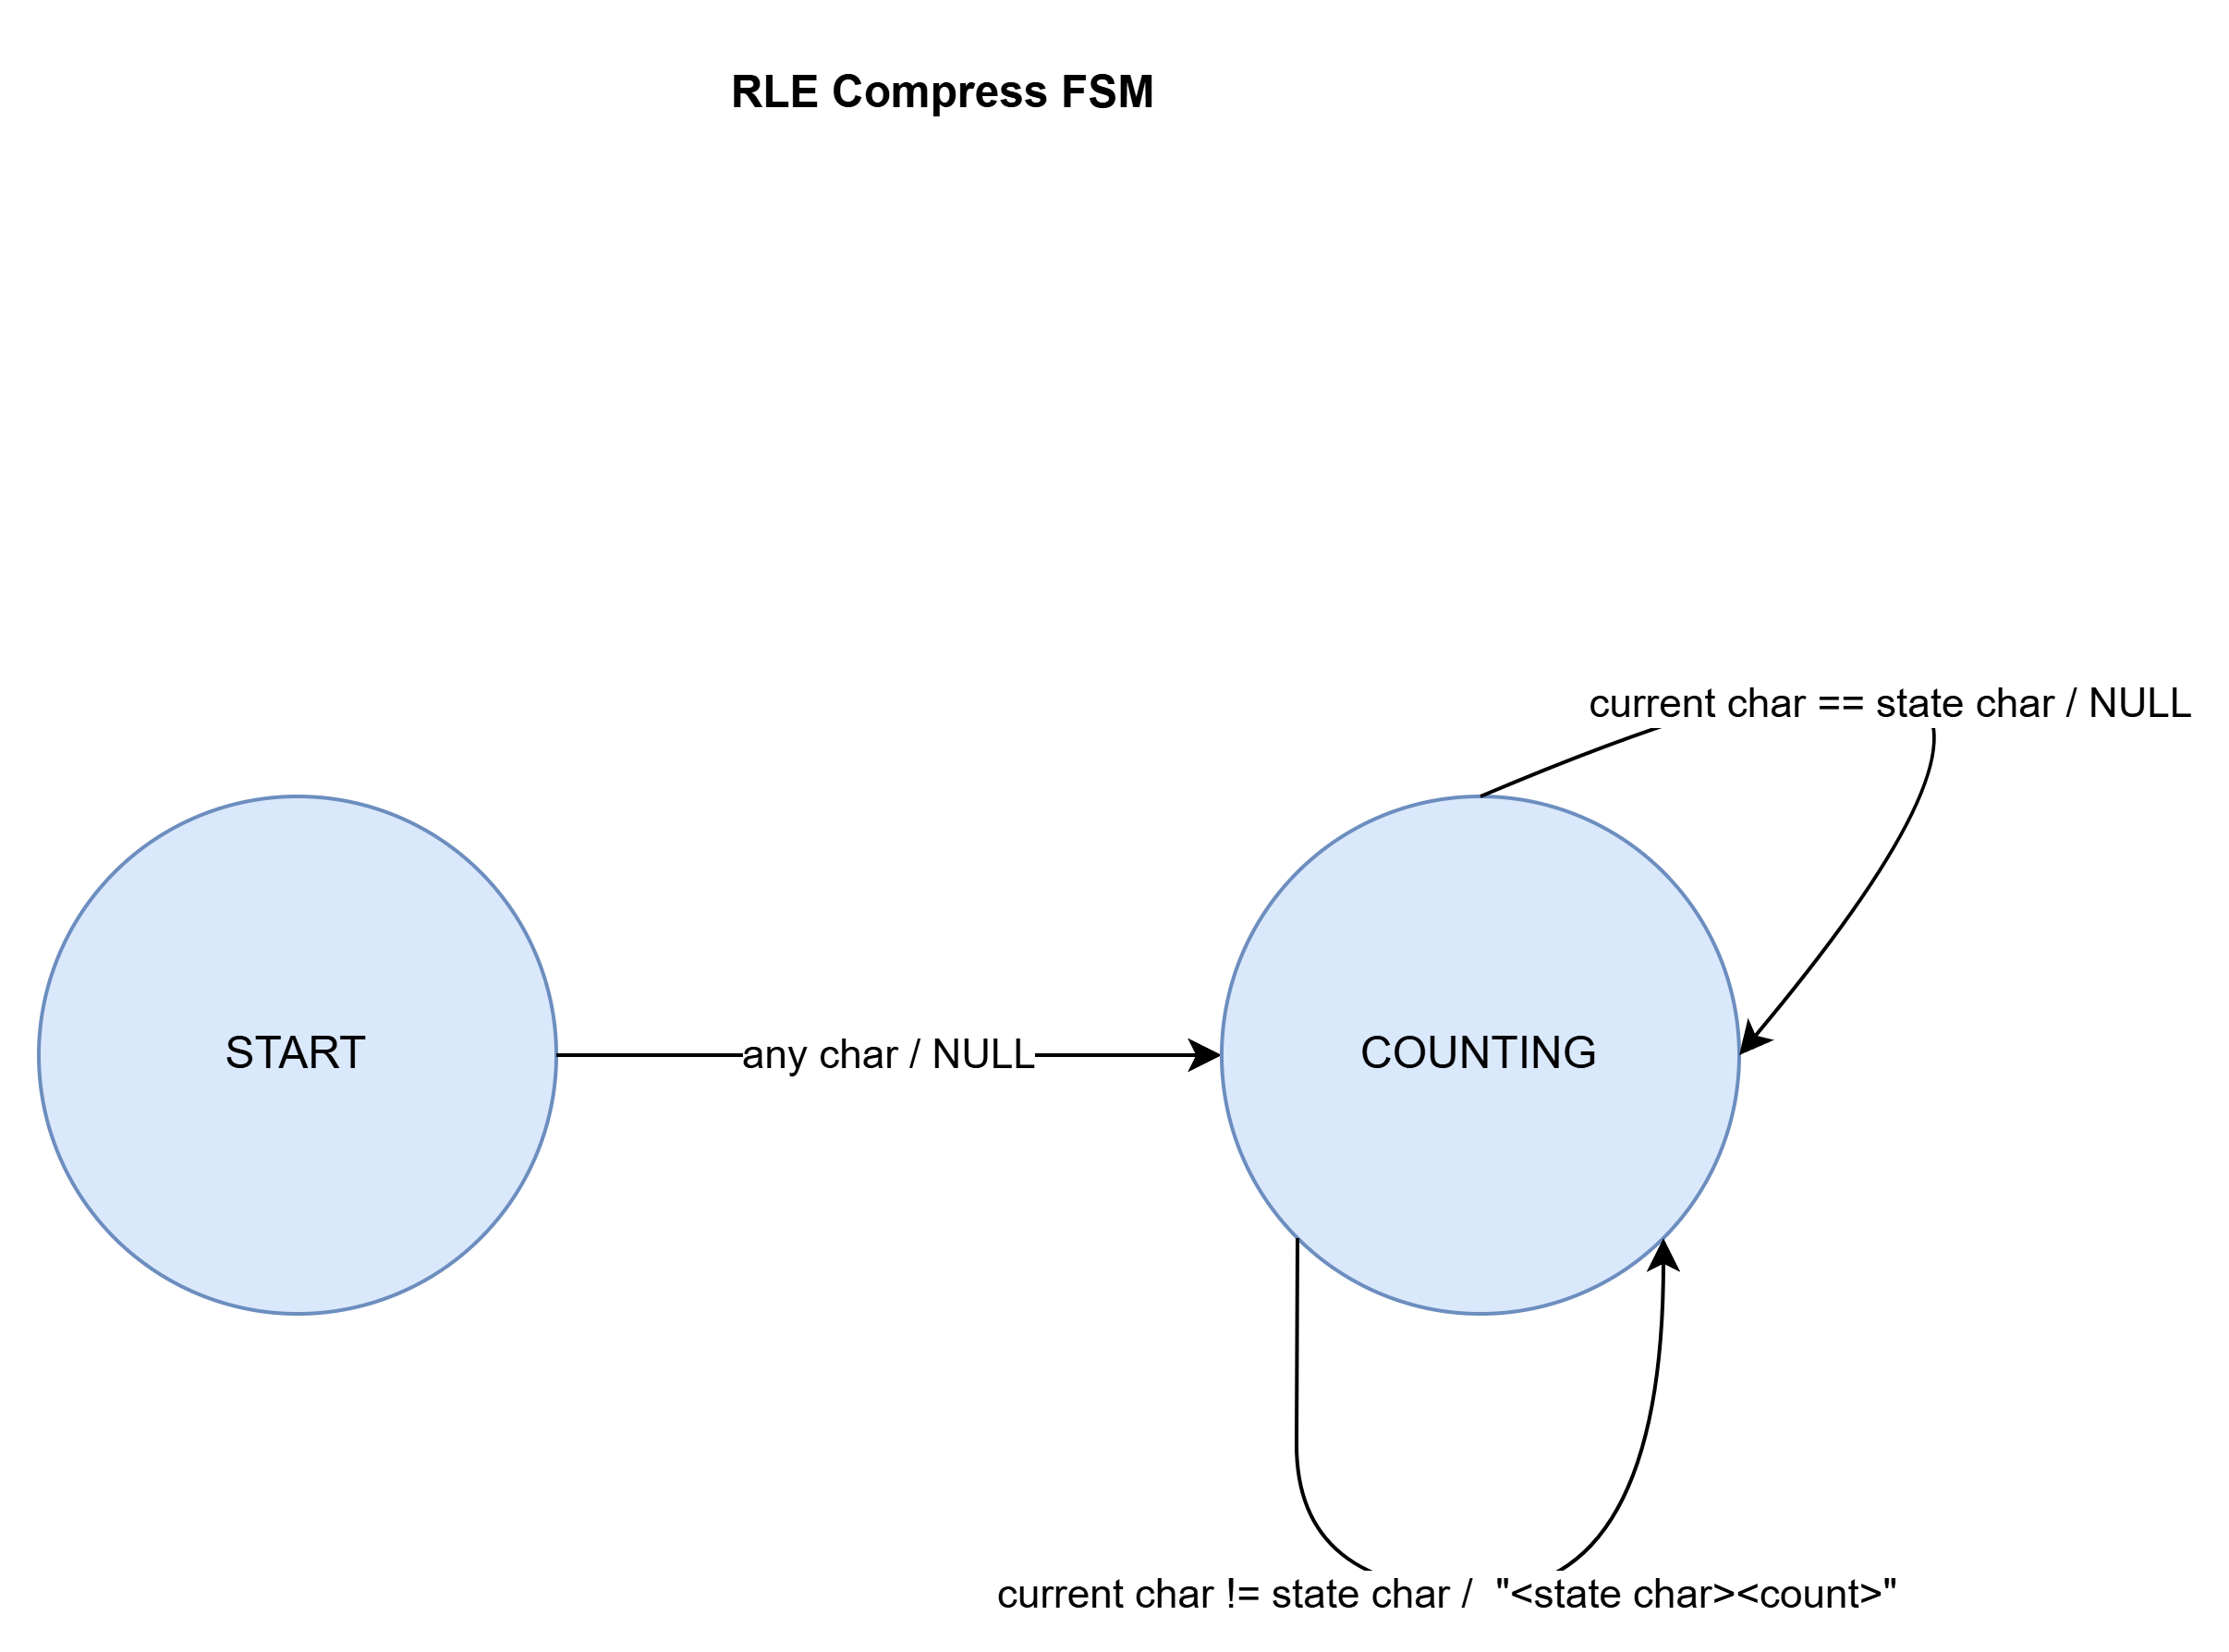
\includegraphics[height=4.5cm]{figures/rle_compress_fsm.png}
        \caption{RLE Compress FSM}
        \label{fig:rle-com-fsm}
    \end{subfigure}
    \hfill
    \begin{subfigure}[t]{0.48\linewidth}
        \centering
        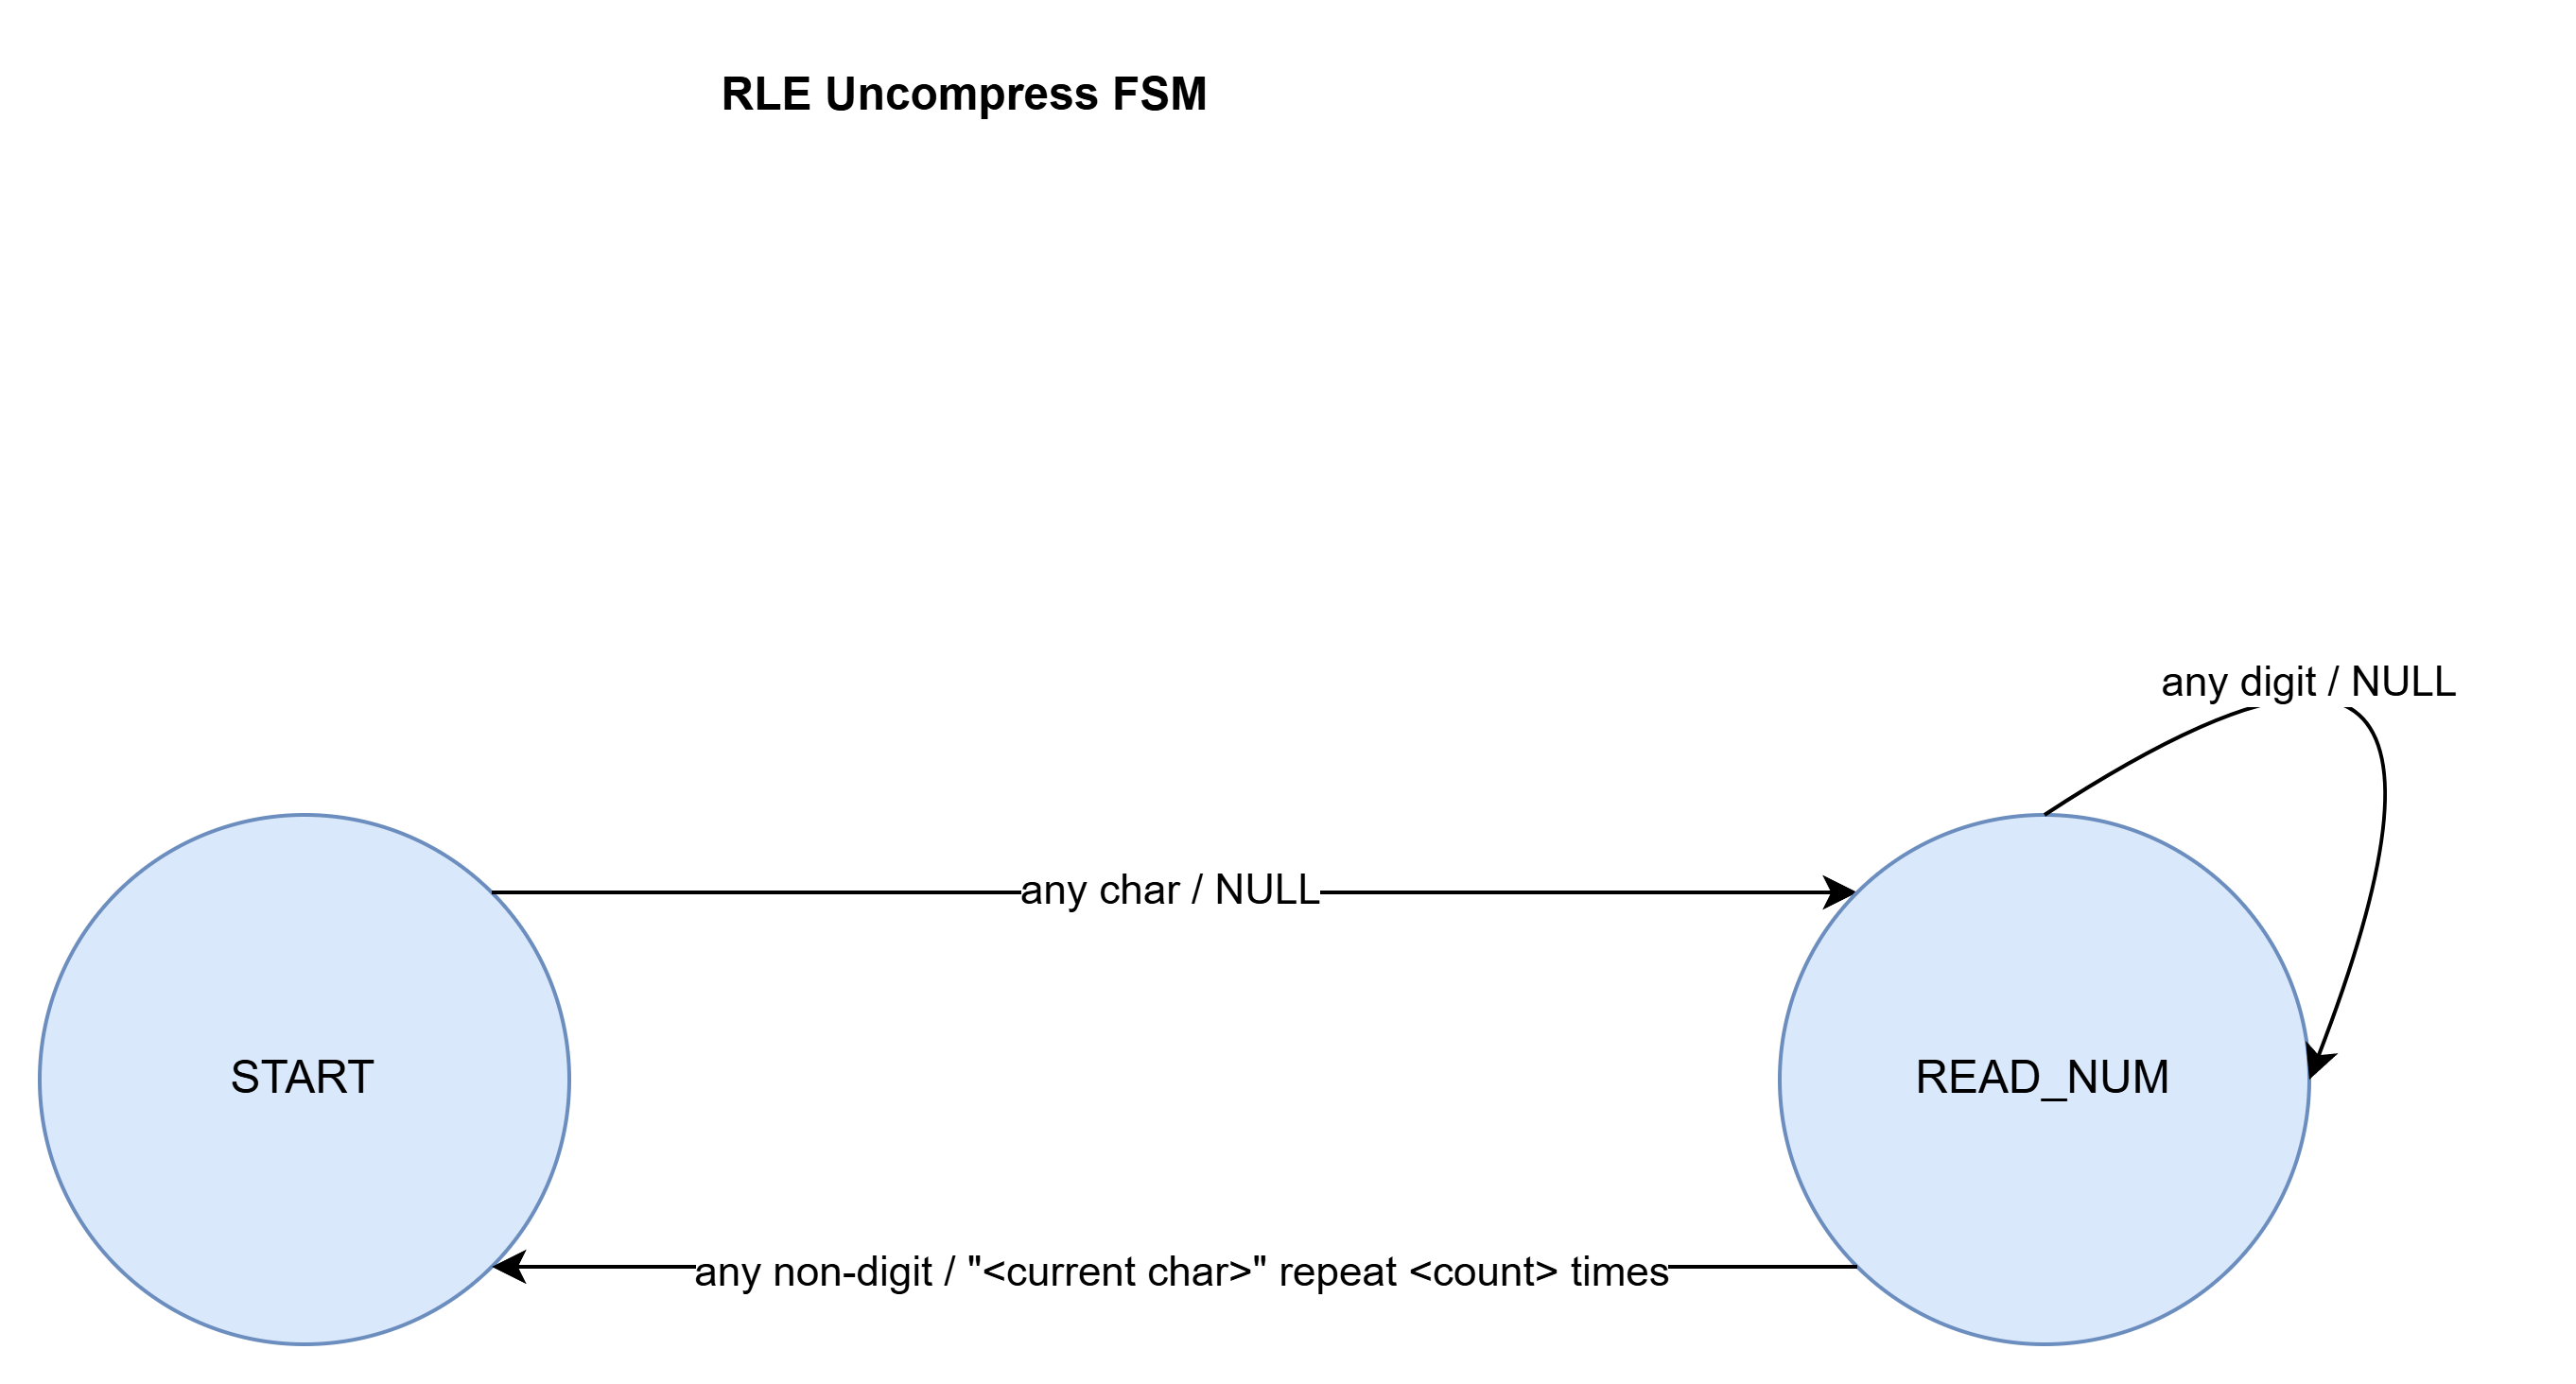
\includegraphics[height=4.3cm]{figures/rle_decompress_fsm.png}
        \caption{RLE Decompress FSM}
        \label{fig:rle-decom-fsm}
    \end{subfigure}

    \caption{RLE Compression and Decompression FSMs}
    \label{fig:rle-fsms}
\end{figure}

\noindent The Run-Length Encoding (RLE) compression and decompression processes are implemented using finite state machines (FSMs), as shown in Figures~\ref{fig:rle-com-fsm} and~\ref{fig:rle-decom-fsm}.

\vspace{0.3em}
\noindent For \textbf{compression}, the FSM has two states: \textit{Start} and \textit{Counting}. The first character initializes a run, after which consecutive identical characters are counted. When a different character is encountered, the current run is encoded as a character–count pair and appended to the output, and a new run begins. After processing the input, the final run is written. This approach performs compression in a single pass.

\vspace{0.3em}
\noindent For \textbf{decompression}, the FSM consists of three states: \textit{Start}, \textit{Read Number}, and \textit{Write}. A character is first read and stored, followed by digits that form its run length. Once the number is complete, the character is repeated accordingly and written to the output. The FSM then returns to the Start state to process the next segment, with checks to handle invalid inputs.

\subsubsection{Delta Encoding}
Delta encoding is applied across consecutive ASCII frames produced by the renderer. Instead of storing each frame independently, the algorithm encodes only the differences between the current frame and the previous frame. This exploits temporal redundancy, as \textbf{consecutive frames in a video are often highly similar}. The first frame is stored in its original form, as there is no prior reference frame for comparison.

\vspace{0.5em}
\noindent\textbf{Example} \newline
Frame 1: AAAAABBBBBCCCC \newline
Frame 2: AAAAADDDEECCCC \newline
\[
\begin{aligned}
Frame_1 &\xrightarrow{\text{Delta encoding}} Frame_1  \\
Frame_2 &\xrightarrow{\text{Delta encoding}} \text{=5+5DDDEE=5}
\end{aligned}
\]
where:
\begin{itemize}
    \item \textbf{=n} indicates that the next $n$ characters are identical to those in the previous frame
    \item \textbf{+n[substring]} indicates that the next n characters differ from the previous frame and are replaced by the specified substring from the current frame.
\end{itemize}

\vspace{0.5em}
\noindent\textbf{FSMs} \newline
\begin{figure}[H]
    \centering
    
    \begin{subfigure}[t]{0.48\linewidth}
        \centering
        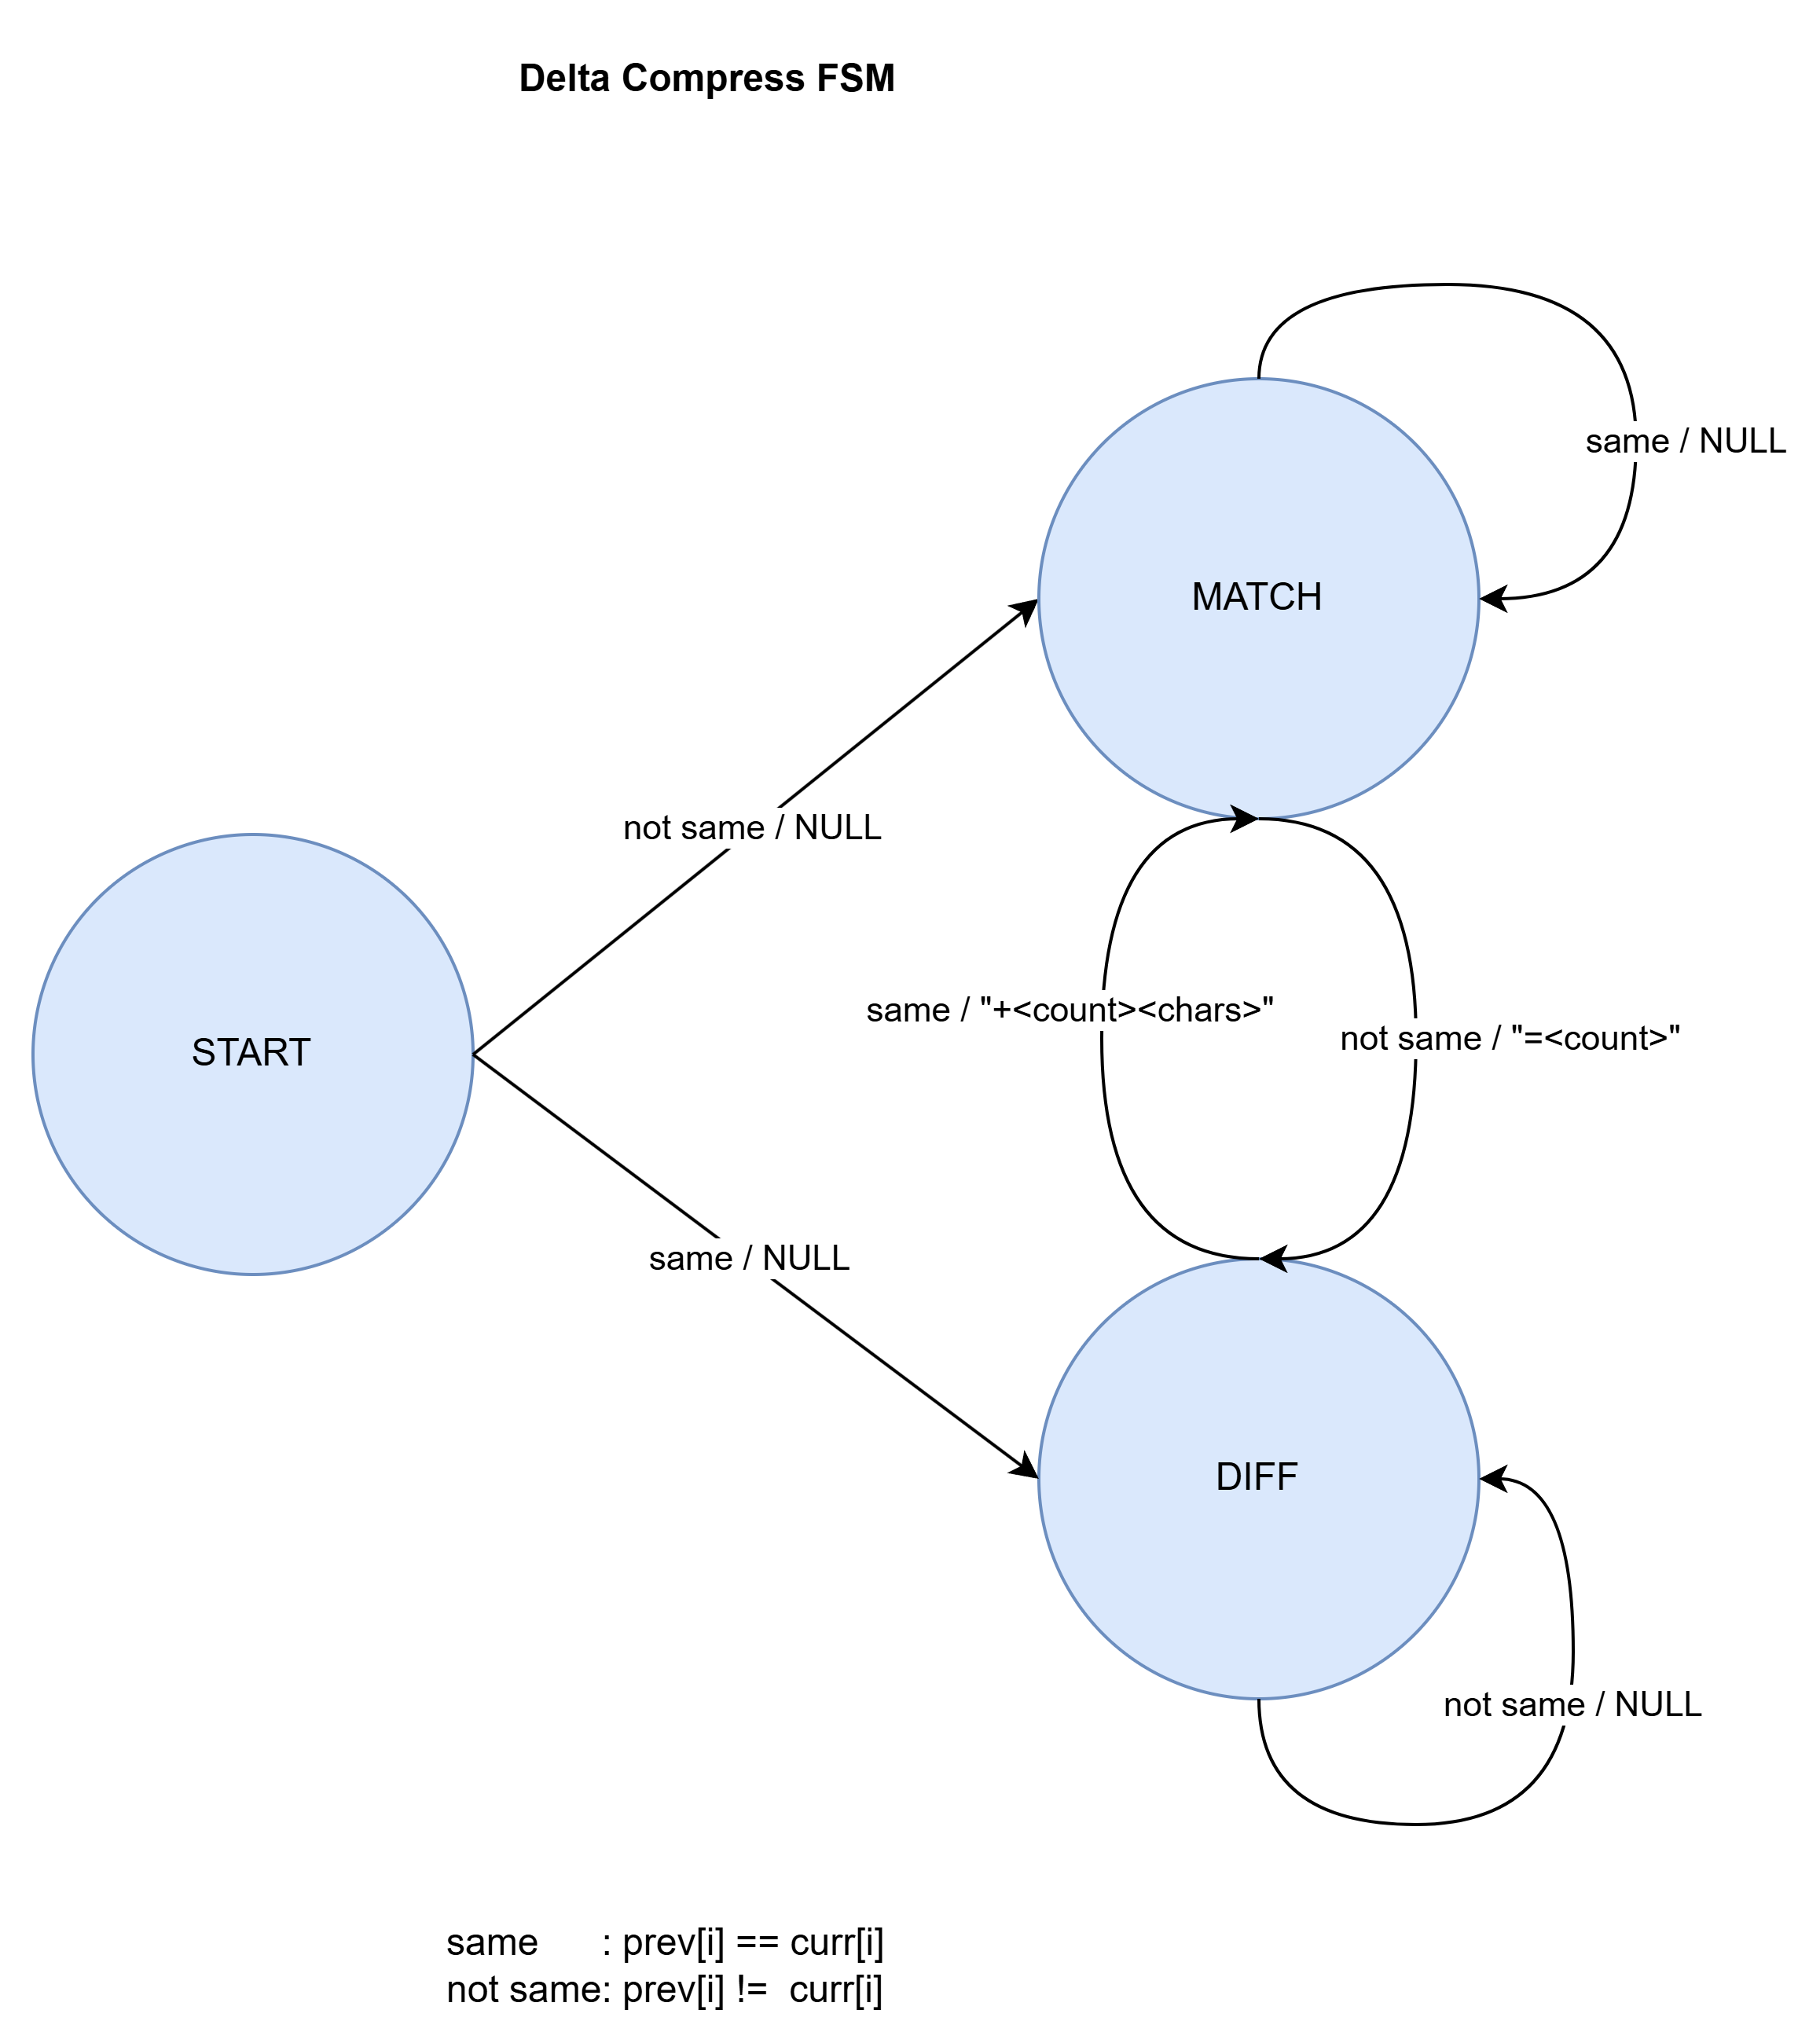
\includegraphics[height=6.5cm]{figures/delta_compress_fsm.png}
        \caption{Delta Compress FSM}
        \label{fig:delta-com-fsm}
    \end{subfigure}
    \hfill
    \begin{subfigure}[t]{0.48\linewidth}
        \centering
        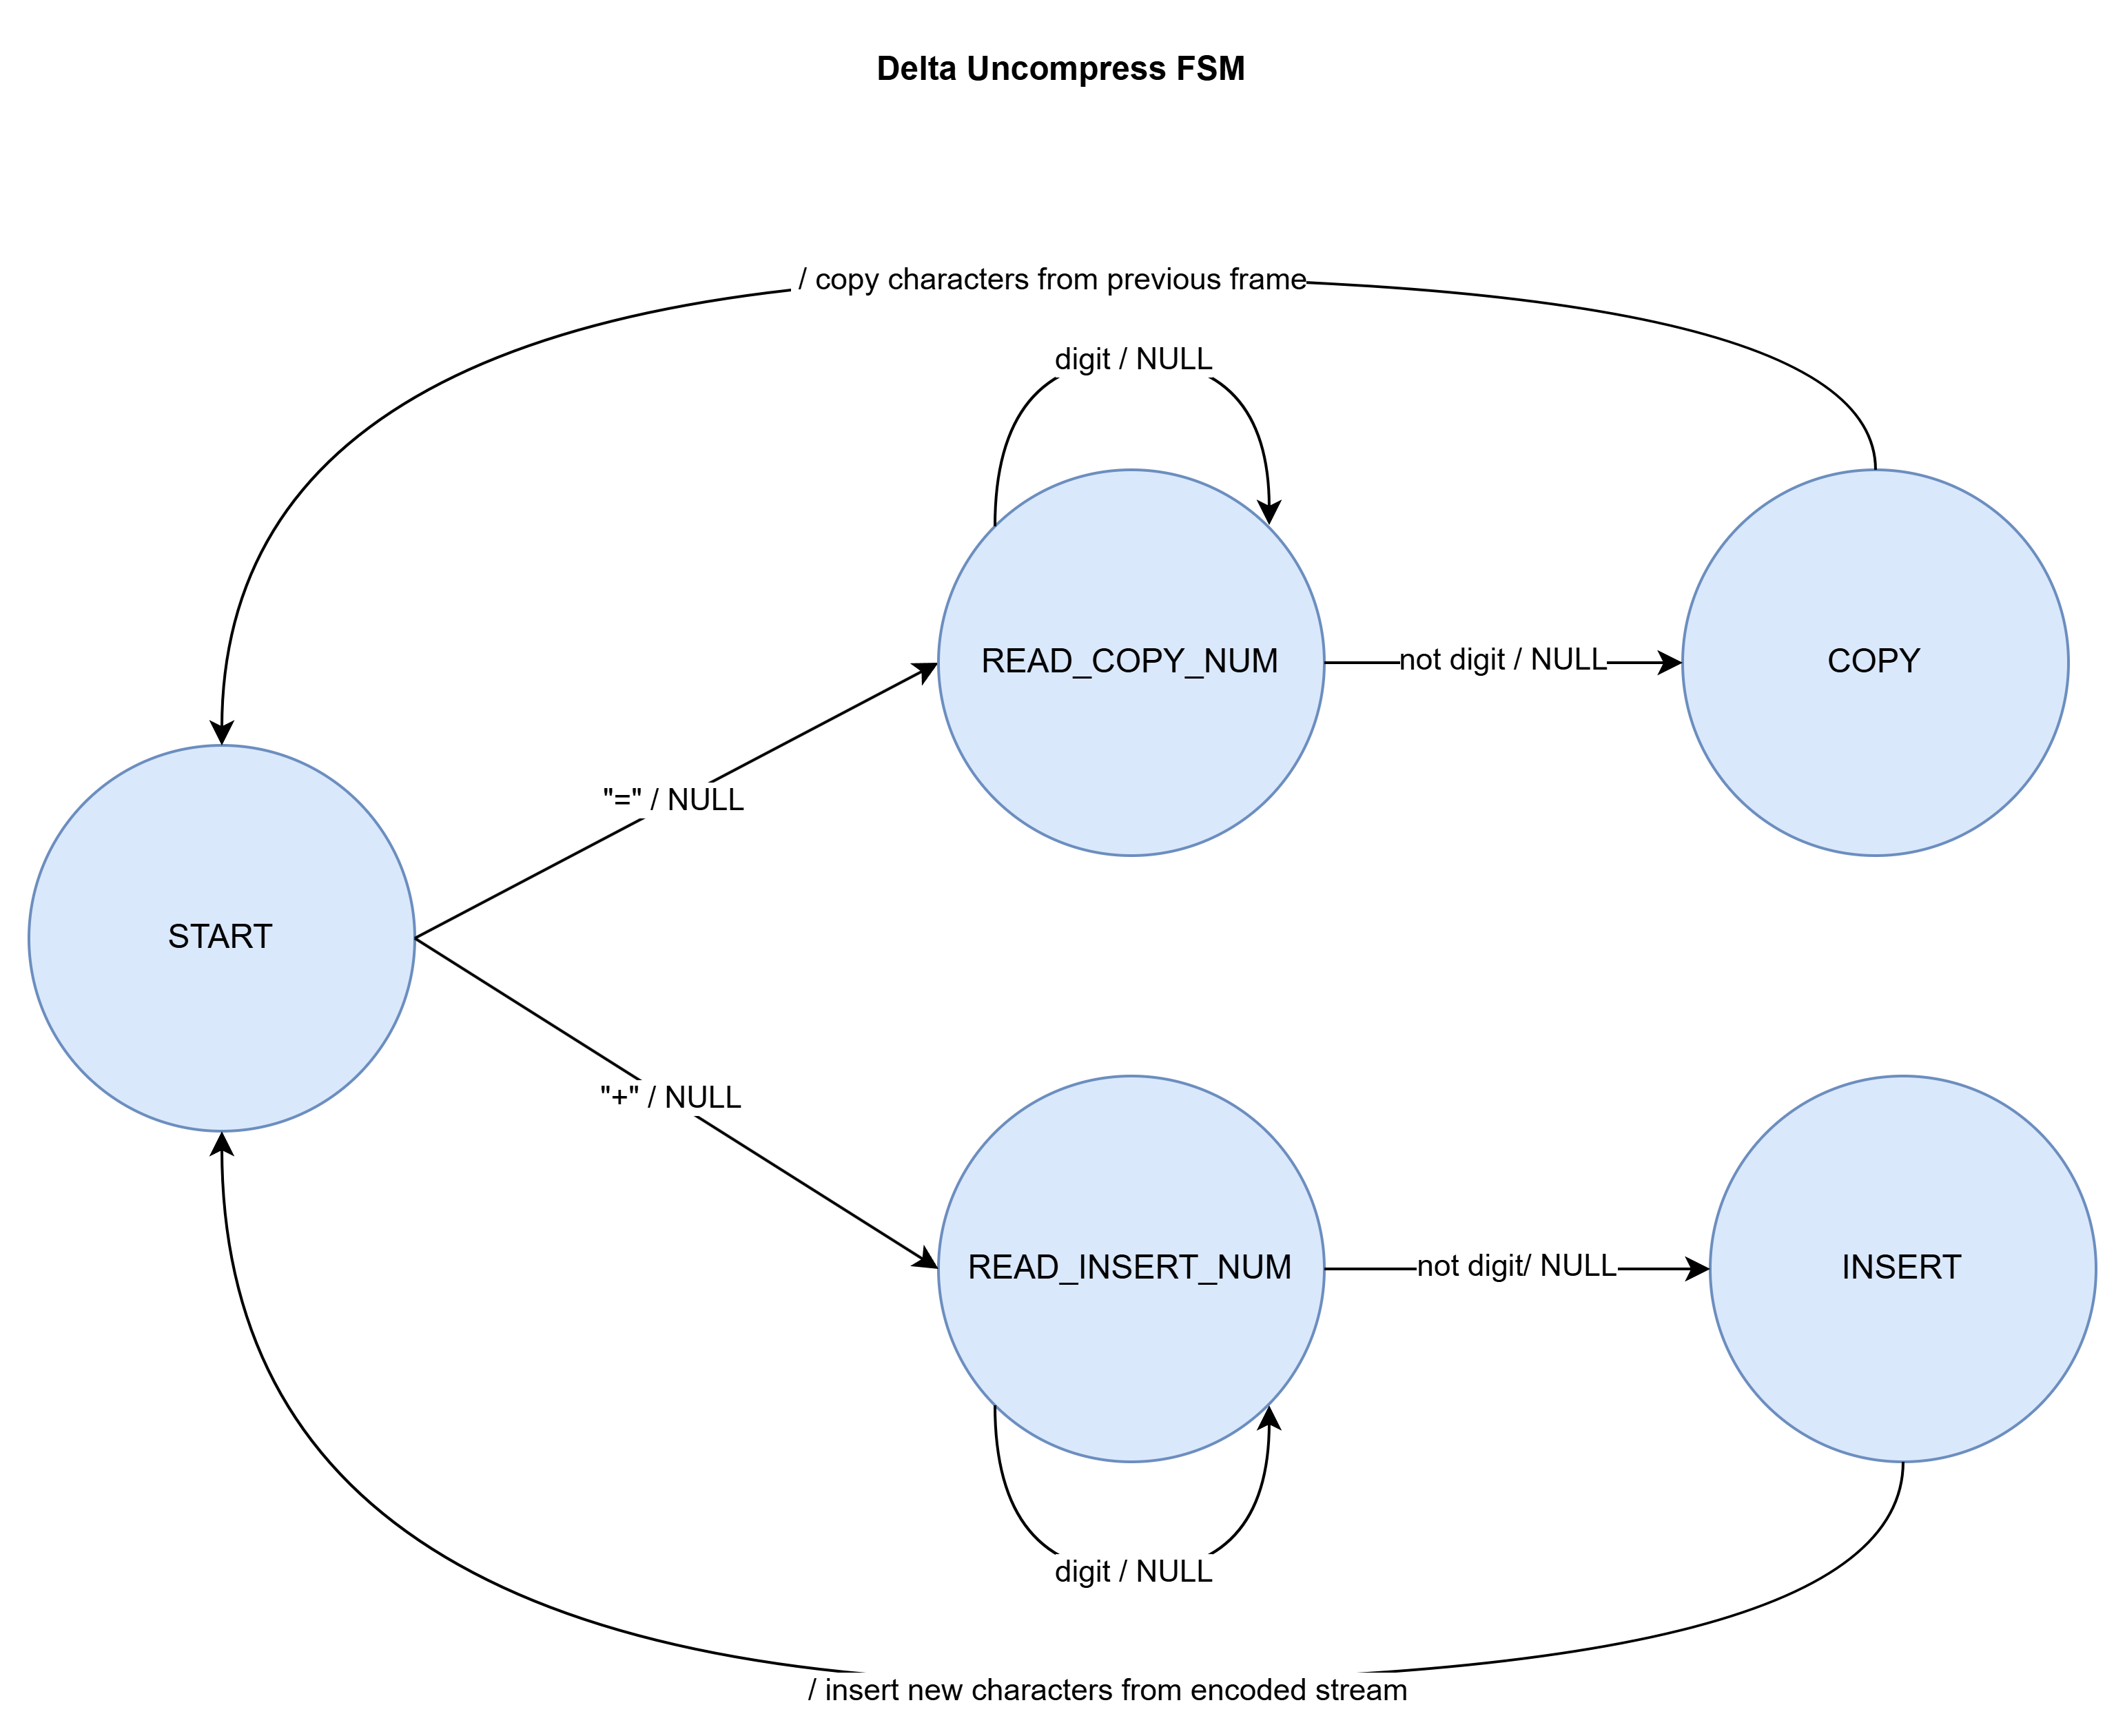
\includegraphics[height=6.5cm]{figures/delta_decompress_fsm.png}
        \caption{Delta Decompress FSM}
        \label{fig:delta-decom-fsm}
    \end{subfigure}

    \caption{Delta Compression and Decompression FSMs}
    \label{fig:delta-fsms}
\end{figure}
\noindent The Delta compression and decompression processes are implemented using finite state machines (FSMs), as shown in Figures~\ref{fig:delta-com-fsm} and~\ref{fig:delta-decom-fsm}.

\vspace{0.3em}
\noindent For \textbf{compression}, the FSM consists of three states: \textit{Start}, \textit{Match}, and \textit{Diff}. The algorithm compares the current frame with a reference (previous) frame character by character. In the Match state, consecutive identical characters are grouped and encoded as a copy operation. In the Diff state, differing characters are grouped and encoded as an insertion. The FSM transitions between these states whenever the comparison result changes, ensuring that both matching and differing segments are efficiently encoded in a single pass.

\vspace{0.3em}
\noindent For \textbf{decompression}, the FSM operates with states \textit{Start}, \textit{Read Copy Number}, \textit{Read Insert Number}, \textit{Copy}, and \textit{Insert}. The encoded stream is parsed by first identifying whether the next operation is a copy or insert. The corresponding run length is then read, after which characters are either copied from the reference frame or inserted directly from the encoded input. The FSM repeats this process until the entire output is reconstructed, with checks to ensure the encoded format is valid.    

\subsubsection{Huffman Coding}

\noindent Huffman coding is a variable-length encoding technique that assigns shorter bit sequences to more frequent symbols and longer sequences to less frequent ones. Unlike RLE and Delta encoding, which operate directly on characters, Huffman coding produces a \textbf{bit stream} to achieve compression beyond the limits of ASCII representation.

\vspace{0.5em}
\noindent \textbf{Huffman Coding without FSM}  \newline
\noindent The standard approach consists of two stages: tree construction and encoding/decoding. A Huffman tree is first built using symbol frequencies, where each leaf node represents a character and the path from the root defines its binary code. Encoding is performed by replacing each character with its corresponding bit sequence, while decoding traverses the tree bit by bit until a leaf node is reached. 

\vspace{0.3em}
\noindent \textbf{Example} \\

\noindent Original text: \texttt{AAAAABBBCC}

\medskip
\noindent \textbf{Step 1: Compute frequency of each character.}

\begin{table}[H]
\centering
\begin{tabular}{c|c}
\textbf{Character} & \textbf{Frequency} \\
\hline
A & 5 \\
B & 3 \\
C & 2 \\
\end{tabular}
\caption{Huffman Frequency Table for \texttt{AAAAABBBCC}}
\label{tab:huffman-freq}
\end{table}

\noindent The frequencies determine how the Huffman tree is constructed, where less frequent symbols are placed deeper in the tree.

\medskip
\noindent \textbf{Step 2: Build the Huffman tree.}

\begin{figure}[H]
    \centering
    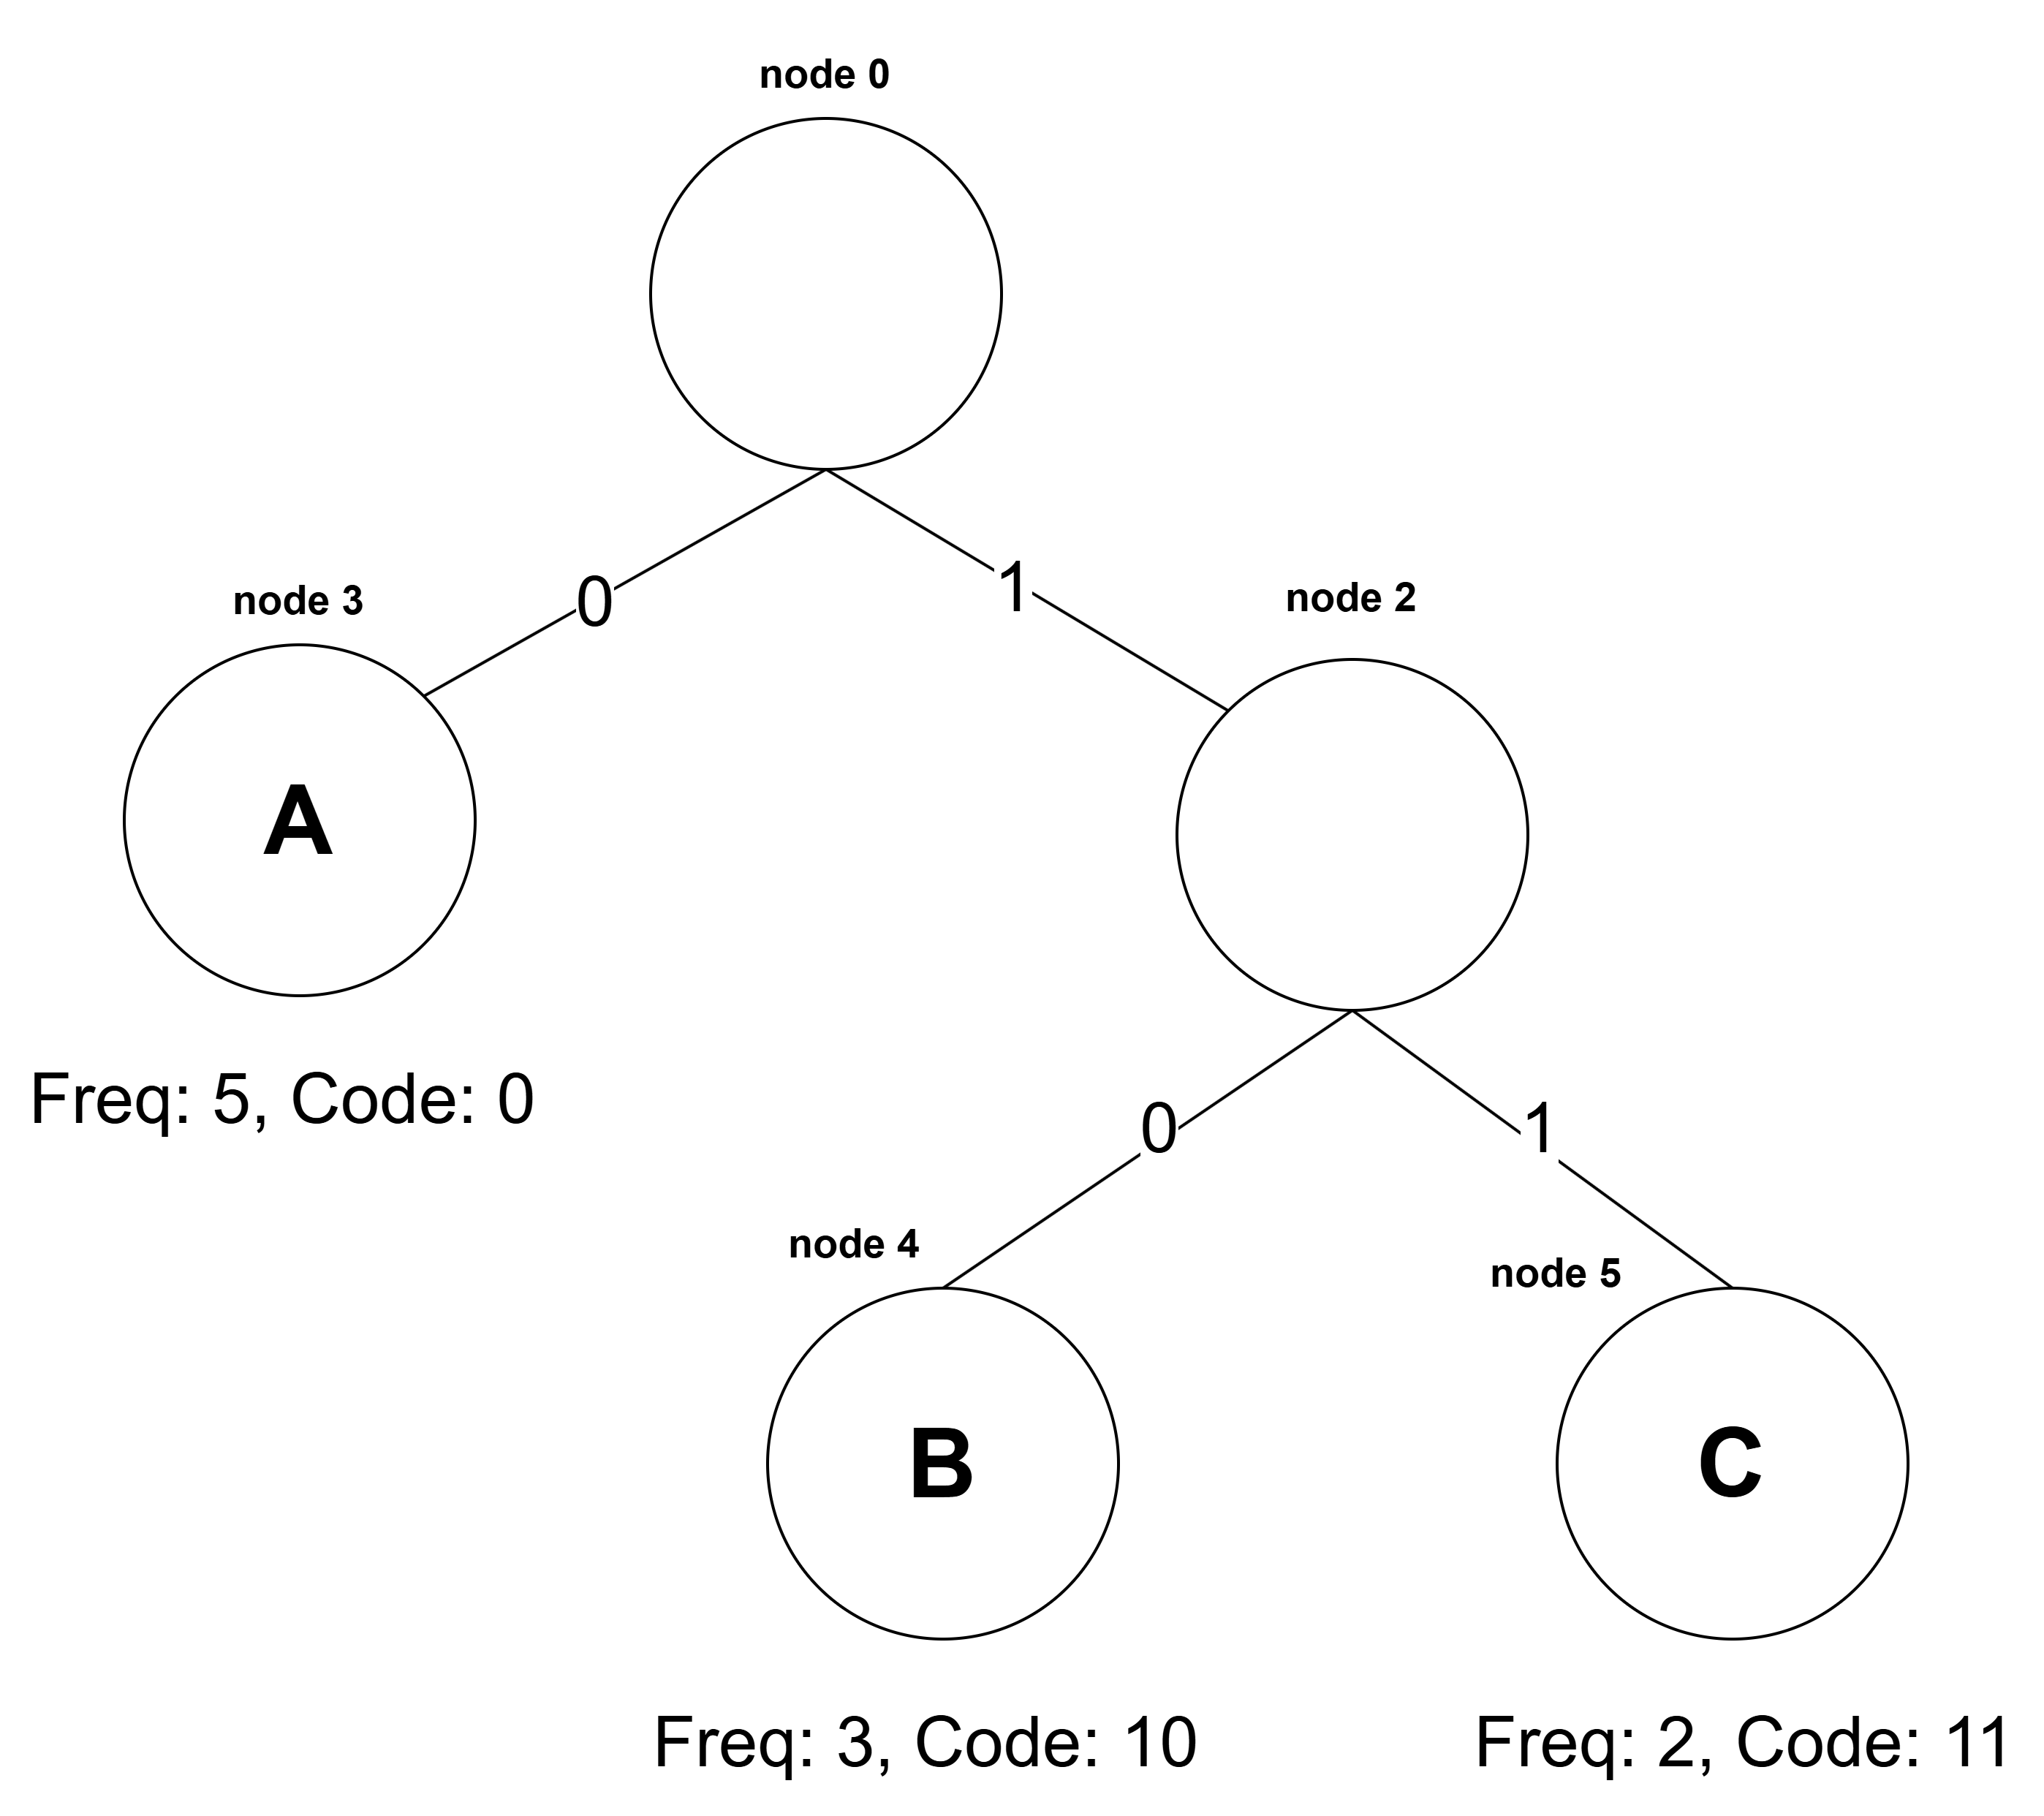
\includegraphics[width=0.5\linewidth]{figures/huffman_tree.png}
    \caption{Huffman Tree for \texttt{AAAAABBBCC}}
    \label{fig:huffman-tree}
\end{figure}

\noindent The Huffman tree is constructed using a greedy approach with a min-heap data structure. First, all characters with non-zero frequencies are inserted into the heap as individual leaf nodes, where each node stores a character and its frequency.

\vspace{0.3em}
\noindent At each step, the two nodes with the smallest frequencies are extracted from the heap. These two nodes are then merged to form a new internal node, whose frequency is the sum of the two. The extracted nodes become the left and right children of this new node. The merged node is then inserted back into the heap.

\vspace{0.3em}
\noindent This process is repeated until only one node remains in the heap, which becomes the root of the Huffman tree. The resulting tree ensures that characters with higher frequencies are closer to the root, leading to shorter binary codes.

\medskip
\noindent \textbf{Step 3: Encode the text using the generated codes.}

\[
\texttt{AAAAABBBCC}
\;\xrightarrow{\text{Huffman coding}}\;
00000\;101010\;1111
\]

\noindent Each character is replaced by its corresponding binary code obtained from the Huffman tree. This is done by traversing from the root to the leaf node of each character, appending a `0` for a left edge and a `1` for a right edge. The resulting codes are concatenated to form a continuous bit stream.

\vspace{0.3em}
\noindent Since more frequent characters have shorter codes, the overall length of the encoded bit stream is reduced compared to fixed-length representations such as ASCII. The bit stream is stored using a bit-level buffer rather than characters, allowing efficient packing of bits into bytes.

\medskip
\noindent \textbf{Step 4: Decode the bit stream.}

\noindent The encoded bit stream is decoded by traversing the Huffman tree from the root according to each bit. A `0` corresponds to moving to the left child, while a `1` corresponds to moving to the right child. When a leaf node is reached, the corresponding character is emitted, and traversal restarts from the root for the next sequence of bits.

\noindent For example, the bit stream
\[
00000\;101010\;1111
\]
is decoded by repeatedly following paths in the tree, reconstructing the original text:
\[
\texttt{AAAAABBBCC}
\]

\noindent In practice, the bit stream is read using a bit-level reader, which extracts bits from the compressed byte array. The decoding process requires processing one bit at a time, resulting in a time complexity of $O(N)$ with relatively \textbf{high constant overhead} due to frequent tree traversal. \\

\noindent \textbf{Optimization: Huffman Decoding with FSM}

\noindent To reduce the overhead of bit-by-bit tree traversal, the Huffman decoding process can be optimized using a finite state machine (FSM). Instead of processing one bit at a time, the FSM reads $K$ bits in each step and performs a table lookup to determine the output symbols and next state.

\medskip
\noindent \textbf{Step 1: Convert the Huffman tree into an FSM.}

\noindent Each internal node in the Huffman tree is treated as a state. For a given state, all possible $2^K$ bit combinations are precomputed. Each entry stores:
\begin{itemize}
    \item the sequence of decoded characters,
    \item the number of bits consumed,
    \item the next state.
\end{itemize}


\noindent This flattens multiple levels of tree traversal into a single transition.

\medskip
\noindent \textbf{Step 2: Process $K$ bits at a time.}

\vspace{0.3em}
\noindent Instead of reading one bit, the decoder reads $K$ bits from the bit stream and uses them as an index into the FSM table. This allows multiple characters to be decoded in a single step, skipping intermediate tree traversal.

\medskip
\noindent \textbf{Simplified example with $K=2$}

\begin{table}[H]
\centering
\begin{tabular}{c|c|c|c|c}
\textbf{State} & \textbf{Input} & \textbf{Output} & \textbf{Next State} & \textbf{Bits Used} \\
\hline
S0 (Root) & 00 & AA & S0 & 2 \\
S0 (Root) & 01 & A  & S1 & 1 \\
S0 (Root) & 10 & B  & S0 & 2 \\
S0 (Root) & 11 & C  & S0 & 2 \\
\hline
S1 (Root.right) & 00 & BA & S0 & 2 \\
S1 (Root.right) & 01 & B  & S1 & 2 \\
S1 (Root.right) & 10 & C  & S0 & 2 \\
S1 (Root.right) & 11 & C  & S1 & 2 \\
\end{tabular}
\caption{Huffman FSM transition table for $K=2$ with bit consumption}
\end{table}

\noindent \textit{Note1}: Only non-terminal nodes are included as FSM states, since reaching a leaf node results in symbol emission and an immediate reset to the root, making leaf nodes transient and unnecessary as explicit states.

\noindent \textit{Note 2}: Although each transition is selected using a $K$-bit input, the number of bits consumed may be less than $K$. This occurs when a symbol is fully decoded before all $K$ bits are used, leaving the remaining bits to be processed in the next step.

\begin{figure}[H]
    \centering
    
    \begin{subfigure}[t]{0.48\linewidth}
        \centering
        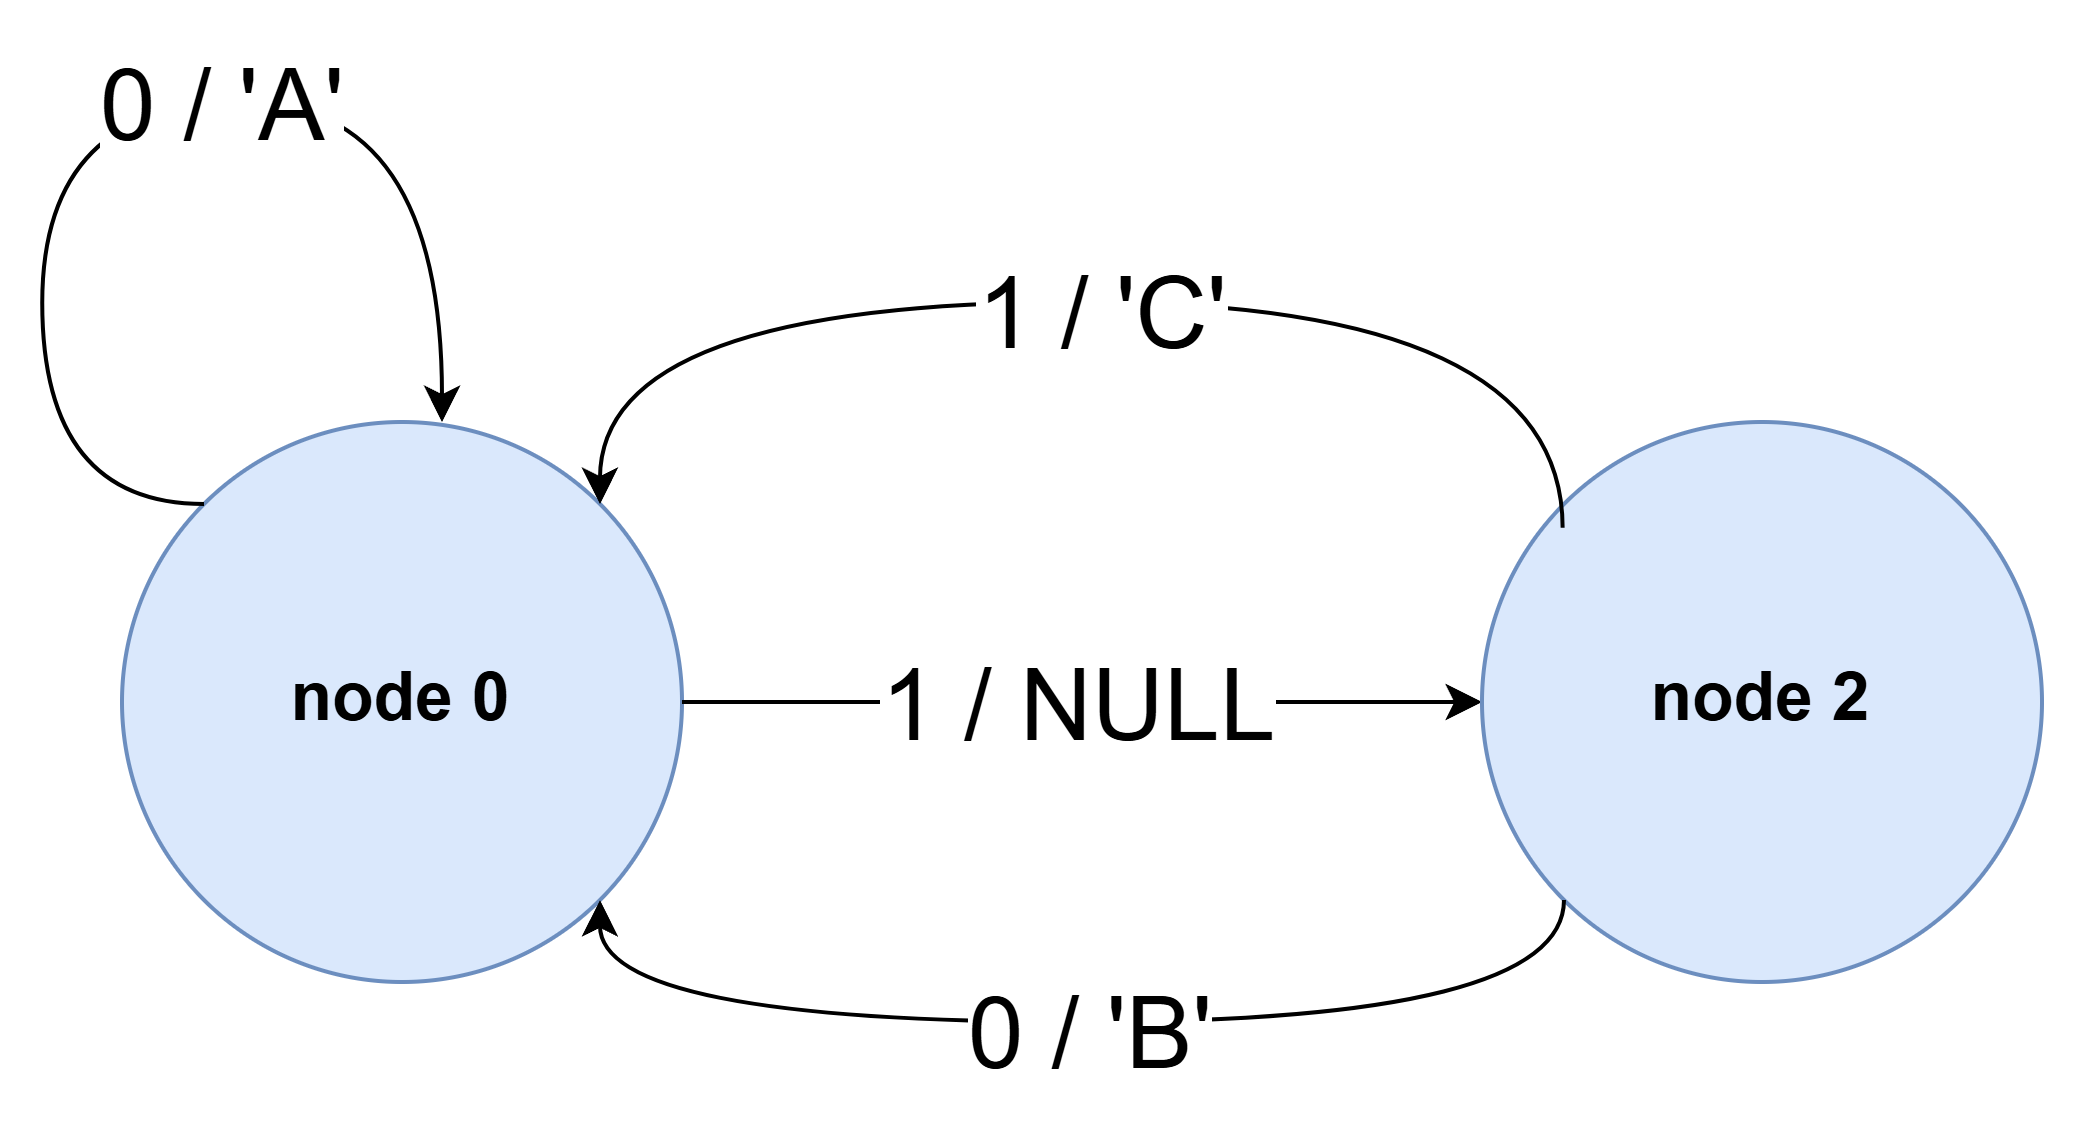
\includegraphics[height=3.5cm]{figures/ori_huffman_fsm.png}
        \caption{Original Huffman FSM ($K=1$)}
        \label{fig:ori-huffman-fsm}
    \end{subfigure}
    \hfill
    \begin{subfigure}[t]{0.48\linewidth}
        \centering
        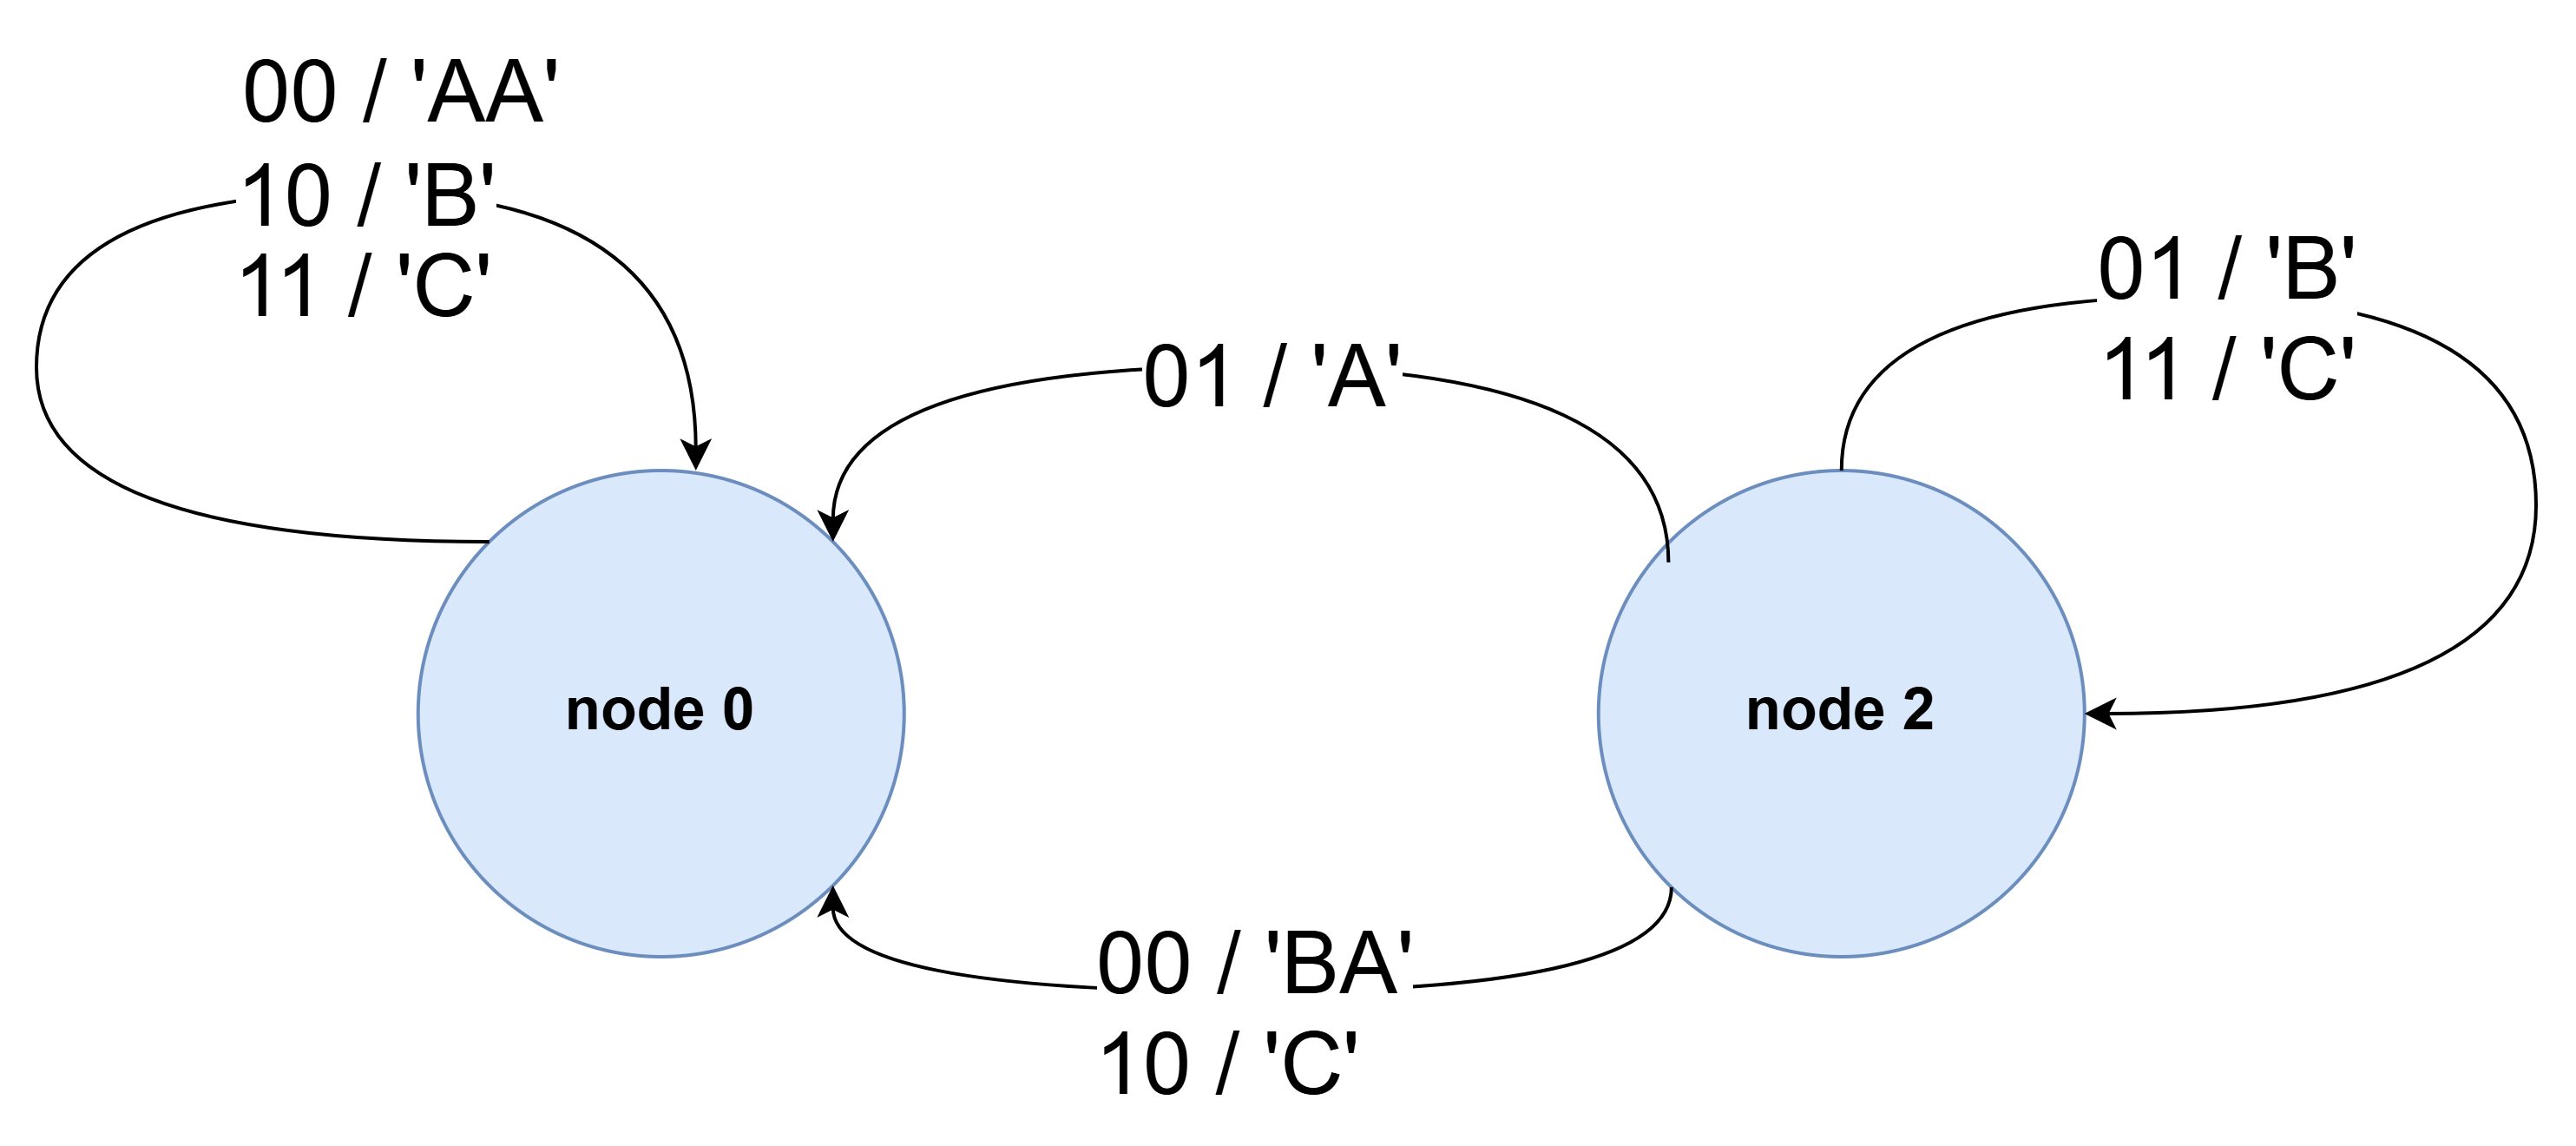
\includegraphics[height=3.5cm]{figures/opt_huffman_fsm.png}
        \caption{Optimized Huffman FSM ($K=2$)}
        \label{fig:opt-huffman-fsm}
    \end{subfigure}

    \caption{Comparison between standard and $K=2$ Huffman decoding FSMs}
    \label{fig:huffman-fsm-comparison}
\end{figure}

\noindent Figure~\ref{fig:huffman-fsm-comparison} compares standard bit-by-bit Huffman decoding with the optimized $K=2$ FSM approach. In the original FSM, each transition processes a single bit, producing \textbf{one character at a time} and incurring higher overhead due to repeated tree traversal.

\vspace{0.3em}
\noindent In contrast, the optimized FSM \textbf{processes $K=2$ bits per transition}, combining multiple traversal steps into a single table lookup. This allows multiple characters to be emitted in one step, reducing the number of transitions required.
\vspace{0.3em}

\noindent For example, consider the bit stream
\[
000001010101111
\]

\noindent The decoding proceeds as follows (for $K=2$ lookahead):

\[
\begin{aligned}
&\underline{00}0001010101111 \;\rightarrow\; (AA,\;2,\;S0) \\
&\underline{00}01010101111 \;\rightarrow\; (AA,\;2,\;S0) \\
&\underline{01}010101111 \;\rightarrow\; (A,\;1,\;S1) \\
&\underline{10}10101111 \;\rightarrow\; (B,\;2,\;S0) \\
&\underline{10}101111 \;\rightarrow\; (B,\;2,\;S0) \\
&\underline{10}1111 \;\rightarrow\; (B,\;2,\;S0) \\
&\underline{11}11 \;\rightarrow\; (C,\;2,\;S0) \\
&\underline{11} \;\rightarrow\; (C,\;2,\;S0)
\end{aligned}
\]
\noindent Each tuple $(\text{output},\;\text{bits\_used},\;\text{next\_state})$ represents the result of one FSM transition.

\noindent The decoded output is:
\[
\texttt{AAAAABBBCC}
\]


\noindent Each transition is selected using a $K$-bit lookahead, but may consume fewer than $K$ bits. For instance, ``01'' produces ``A'' while consuming only 1 bit, leaving the remaining bit to be processed in the next step. This allows the decoder to combine multiple traversal steps into a single lookup, improving efficiency compared to standard bit-by-bit decoding.

\medskip
\noindent \textbf{Time--space tradeoff}

\vspace{0.3em}
\noindent The FSM-based approach reduces decoding overhead by replacing repeated tree traversal with constant-time table lookups, resulting in faster practical performance. While the overall time complexity remains $O(N)$, the number of decoding steps is reduced to approximately $O(\frac{N}{K})$.

\vspace{0.3em}
\noindent However, this comes at the cost of increased memory usage. The FSM requires a lookup table of size $O(2^K \cdot S)$, where $S$ is the number of states, corresponding to the total number of internal nodes in the Huffman tree. A larger $K$ improves decoding speed by processing more bits per step, but increases memory exponentially. Conversely, a smaller $K$ reduces memory usage but provides less speedup.


\subsubsection{Compressed Size Comparison}

The following are the compressed results using the ASCII frames and configurations (\url{output/demo/demo_engine/test_config.json}) from this work's GitHub repository.

\begin{table}[H]
\centering
\begin{tabular}{l|r}
\textbf{Method} & \textbf{Size (KB)} \\
\hline
Original & 135,684 \\
RLE & 13,297 \\
Delta & 17,943 \\
Huffman $(K=1)$ & 36,885 \\
Huffman $(K=5)$ & 36,893 \\
Huffman $(K=10)$ & 37,251 \\
\end{tabular}
\caption{Compressed size comparison across different algorithms and configurations}
\label{tab:compression-size}
\end{table}

\noindent \textbf{Analysis.}

\begin{itemize}
    \item \textit{RLE}: Achieves the best compression, reducing the data size by an order of magnitude. This is due to long runs of identical characters across consecutive frames, which RLE encodes very efficiently.

    \item \textit{Delta encoding}: Performs well since consecutive frames are largely similar. By encoding only the differences, it reduces inter-frame redundancy. However, these differences are often scattered rather than continuous, making it less effective than RLE.

    \item \textit{Huffman coding}: Performs worse in this case. The character distribution is relatively uniform, limiting the benefit of variable-length encoding. Additionally, it operates at the symbol (character) level and does not exploit redundancy across frames. For the FSM-based optimization, increasing $K$ introduces exponential memory overhead ($O(2^K)$) without improving compression ratio.
\end{itemize}
